\documentclass[11pt]{article}

% Shared notes settings for Applied Machine Learning lectures (UPES).
% Keep this file free of \documentclass to allow reuse via \input.

\usepackage[utf8]{inputenc}
\usepackage[T1]{fontenc}
\usepackage{lmodern}          % scalable T1 fonts; without this pdflatex falls back
\input{glyphtounicode}        % to bitmapped EC Type 3 and the PDFs are neither
\pdfgentounicode=1            % searchable nor screen-reader friendly
\usepackage[a4paper,margin=1in]{geometry}
\usepackage{hyperref}
\usepackage{xurl}
\usepackage{booktabs}
\usepackage{amsmath}
\usepackage{amssymb}
\usepackage{listings}
\usepackage{xcolor}
\usepackage{enumitem}
\usepackage{parskip}

% Code listings (Python-oriented for this subject).
\lstset{
  language=Python,
  basicstyle=\ttfamily\small,
  keywordstyle=\color{blue},
  commentstyle=\color{gray},
  stringstyle=\color{teal},
  showstringspaces=false,
  columns=fullflexible,
  frame=single,
  framerule=0.2pt,
  breaklines=true
}

\setlist[itemize]{topsep=0.3em,itemsep=0.2em}
\setlist[enumerate]{topsep=0.3em,itemsep=0.2em}

% Simple per-section source line.
\newcommand{\notesources}[1]{\par\noindent{\small\color{gray}\textit{Sources:} \sloppy #1\par}}

% Unit-wise source strings for this subject (used by slides + notes).
% Path is relative to the lecture `latex/` folder (the compilation CWD).
\IfFileExists{../../../_shared/aml-sources.tex}{%
  % Source strings for Applied Machine Learning (CSAI2017P) — used by slides + notes.
% Prescribed texts and reference books are taken from the course syllabus.
% Support texts are the author-hosted open-access editions:
%   statlearning.com            (ISL with Python)
%   probml.github.io/pml-book   (Murphy, Probabilistic Machine Learning)
%   d2l.ai                      (Dive into Deep Learning)
%   mml-book.github.io          (Mathematics for Machine Learning)

\newcommand{\AMLRepoURL}{https://github.com/tali7c/Applied-Machine-Learning}

% --- prescribed -------------------------------------------------------------
\newcommand{\AMLPrescribed}{%
M\"uller and Guido, \textit{Introduction to Machine Learning with Python}, O'Reilly, 2016.;%
Bishop, \textit{Pattern Recognition and Machine Learning}, Springer, 2006.;%
Murphy, \textit{Machine Learning: A Probabilistic Perspective}, MIT Press, 2012.;%
Han, Kamber and Pei, \textit{Data Mining: Concepts and Techniques} (3e), Morgan Kaufmann, 2012.%
}

% --- unit-wise ---------------------------------------------------------------
\newcommand{\AMLUnitISources}{%
M\"uller and Guido, \textit{Introduction to Machine Learning with Python}, Ch. 1.;%
Bishop, \textit{Pattern Recognition and Machine Learning}, Ch. 1.;%
Murphy, \textit{Probabilistic Machine Learning: An Introduction}, MIT Press, 2022, Ch. 1.;%
Mitchell, \textit{Machine Learning}, McGraw Hill, 1997, Ch. 1.;%
Scikit-learn documentation, accessed 2026-08-04.%
}

\newcommand{\AMLUnitIISources}{%
Bishop, \textit{Pattern Recognition and Machine Learning}, \S1.5, \S4.3, \S7.1.;%
Zhang, Lipton, Li and Smola, \textit{Dive into Deep Learning}, \S3.4.;%
Shalev-Shwartz and Ben-David, \textit{Understanding Machine Learning}, Ch. 15.;%
Murphy, \textit{Probabilistic Machine Learning: An Introduction}, Ch. 5.%
}

\newcommand{\AMLUnitIIISources}{%
Zhang, Lipton, Li and Smola, \textit{Dive into Deep Learning}, Ch. 12 (Optimization Algorithms).;%
Deisenroth, Faisal and Ong, \textit{Mathematics for Machine Learning}, Ch. 7.;%
Kingma and Ba, ``Adam: A Method for Stochastic Optimization,'' ICLR 2015.;%
Ruder, ``An overview of gradient descent optimization algorithms,'' arXiv:1609.04747, 2016.%
}

\newcommand{\AMLUnitIVSources}{%
Han, Kamber and Pei, \textit{Data Mining: Concepts and Techniques} (3e), Ch. 3.;%
M\"uller and Guido, \textit{Introduction to Machine Learning with Python}, Ch. 3--4.;%
James, Witten, Hastie, Tibshirani and Taylor, \textit{An Introduction to Statistical Learning with Python}, Ch. 5--6, 12.;%
Scikit-learn documentation (preprocessing, model selection), accessed 2026-08-04.%
}

\newcommand{\AMLUnitVSources}{%
James et al., \textit{An Introduction to Statistical Learning with Python}, Ch. 3--6.;%
Bishop, \textit{Pattern Recognition and Machine Learning}, Ch. 3.;%
Deisenroth, Faisal and Ong, \textit{Mathematics for Machine Learning}, Ch. 9.;%
M\"uller and Guido, \textit{Introduction to Machine Learning with Python}, \S2.3.%
}

\newcommand{\AMLUnitVISources}{%
Han, Kamber and Pei, \textit{Data Mining: Concepts and Techniques} (3e), Ch. 8--9.;%
James et al., \textit{An Introduction to Statistical Learning with Python}, Ch. 8--9.;%
Bishop, \textit{Pattern Recognition and Machine Learning}, Ch. 4--5, 7, 14.;%
Zhang et al., \textit{Dive into Deep Learning}, Ch. 5.%
}

\newcommand{\AMLUnitVIISources}{%
Han, Kamber and Pei, \textit{Data Mining: Concepts and Techniques} (3e), Ch. 10.;%
James et al., \textit{An Introduction to Statistical Learning with Python}, Ch. 12.;%
M\"uller and Guido, \textit{Introduction to Machine Learning with Python}, \S3.5.;%
Ester, Kriegel, Sander and Xu, ``A density-based algorithm for discovering clusters (DBSCAN),'' KDD 1996.%
}

\newcommand{\AMLLabSources}{%
M\"uller and Guido, \textit{Introduction to Machine Learning with Python}, companion notebooks.;%
McKinney, \textit{Python for Data Analysis} (3e), O'Reilly, 2022.;%
Scikit-learn user guide, accessed 2026-08-04.;%
Matplotlib and Seaborn documentation, accessed 2026-08-04.%
}
%
}{%
  % Faculty copies live under `private/` so their compile CWD is different.
  \IfFileExists{../../../../public/_shared/aml-sources.tex}{%
    % Source strings for Applied Machine Learning (CSAI2017P) — used by slides + notes.
% Prescribed texts and reference books are taken from the course syllabus.
% Support texts are the author-hosted open-access editions:
%   statlearning.com            (ISL with Python)
%   probml.github.io/pml-book   (Murphy, Probabilistic Machine Learning)
%   d2l.ai                      (Dive into Deep Learning)
%   mml-book.github.io          (Mathematics for Machine Learning)

\newcommand{\AMLRepoURL}{https://github.com/tali7c/Applied-Machine-Learning}

% --- prescribed -------------------------------------------------------------
\newcommand{\AMLPrescribed}{%
M\"uller and Guido, \textit{Introduction to Machine Learning with Python}, O'Reilly, 2016.;%
Bishop, \textit{Pattern Recognition and Machine Learning}, Springer, 2006.;%
Murphy, \textit{Machine Learning: A Probabilistic Perspective}, MIT Press, 2012.;%
Han, Kamber and Pei, \textit{Data Mining: Concepts and Techniques} (3e), Morgan Kaufmann, 2012.%
}

% --- unit-wise ---------------------------------------------------------------
\newcommand{\AMLUnitISources}{%
M\"uller and Guido, \textit{Introduction to Machine Learning with Python}, Ch. 1.;%
Bishop, \textit{Pattern Recognition and Machine Learning}, Ch. 1.;%
Murphy, \textit{Probabilistic Machine Learning: An Introduction}, MIT Press, 2022, Ch. 1.;%
Mitchell, \textit{Machine Learning}, McGraw Hill, 1997, Ch. 1.;%
Scikit-learn documentation, accessed 2026-08-04.%
}

\newcommand{\AMLUnitIISources}{%
Bishop, \textit{Pattern Recognition and Machine Learning}, \S1.5, \S4.3, \S7.1.;%
Zhang, Lipton, Li and Smola, \textit{Dive into Deep Learning}, \S3.4.;%
Shalev-Shwartz and Ben-David, \textit{Understanding Machine Learning}, Ch. 15.;%
Murphy, \textit{Probabilistic Machine Learning: An Introduction}, Ch. 5.%
}

\newcommand{\AMLUnitIIISources}{%
Zhang, Lipton, Li and Smola, \textit{Dive into Deep Learning}, Ch. 12 (Optimization Algorithms).;%
Deisenroth, Faisal and Ong, \textit{Mathematics for Machine Learning}, Ch. 7.;%
Kingma and Ba, ``Adam: A Method for Stochastic Optimization,'' ICLR 2015.;%
Ruder, ``An overview of gradient descent optimization algorithms,'' arXiv:1609.04747, 2016.%
}

\newcommand{\AMLUnitIVSources}{%
Han, Kamber and Pei, \textit{Data Mining: Concepts and Techniques} (3e), Ch. 3.;%
M\"uller and Guido, \textit{Introduction to Machine Learning with Python}, Ch. 3--4.;%
James, Witten, Hastie, Tibshirani and Taylor, \textit{An Introduction to Statistical Learning with Python}, Ch. 5--6, 12.;%
Scikit-learn documentation (preprocessing, model selection), accessed 2026-08-04.%
}

\newcommand{\AMLUnitVSources}{%
James et al., \textit{An Introduction to Statistical Learning with Python}, Ch. 3--6.;%
Bishop, \textit{Pattern Recognition and Machine Learning}, Ch. 3.;%
Deisenroth, Faisal and Ong, \textit{Mathematics for Machine Learning}, Ch. 9.;%
M\"uller and Guido, \textit{Introduction to Machine Learning with Python}, \S2.3.%
}

\newcommand{\AMLUnitVISources}{%
Han, Kamber and Pei, \textit{Data Mining: Concepts and Techniques} (3e), Ch. 8--9.;%
James et al., \textit{An Introduction to Statistical Learning with Python}, Ch. 8--9.;%
Bishop, \textit{Pattern Recognition and Machine Learning}, Ch. 4--5, 7, 14.;%
Zhang et al., \textit{Dive into Deep Learning}, Ch. 5.%
}

\newcommand{\AMLUnitVIISources}{%
Han, Kamber and Pei, \textit{Data Mining: Concepts and Techniques} (3e), Ch. 10.;%
James et al., \textit{An Introduction to Statistical Learning with Python}, Ch. 12.;%
M\"uller and Guido, \textit{Introduction to Machine Learning with Python}, \S3.5.;%
Ester, Kriegel, Sander and Xu, ``A density-based algorithm for discovering clusters (DBSCAN),'' KDD 1996.%
}

\newcommand{\AMLLabSources}{%
M\"uller and Guido, \textit{Introduction to Machine Learning with Python}, companion notebooks.;%
McKinney, \textit{Python for Data Analysis} (3e), O'Reilly, 2022.;%
Scikit-learn user guide, accessed 2026-08-04.;%
Matplotlib and Seaborn documentation, accessed 2026-08-04.%
}
%
  }{%
    % Question papers live at `private/<family>/<instrument>/`.
    \IfFileExists{../../../public/_shared/aml-sources.tex}{%
      % Source strings for Applied Machine Learning (CSAI2017P) — used by slides + notes.
% Prescribed texts and reference books are taken from the course syllabus.
% Support texts are the author-hosted open-access editions:
%   statlearning.com            (ISL with Python)
%   probml.github.io/pml-book   (Murphy, Probabilistic Machine Learning)
%   d2l.ai                      (Dive into Deep Learning)
%   mml-book.github.io          (Mathematics for Machine Learning)

\newcommand{\AMLRepoURL}{https://github.com/tali7c/Applied-Machine-Learning}

% --- prescribed -------------------------------------------------------------
\newcommand{\AMLPrescribed}{%
M\"uller and Guido, \textit{Introduction to Machine Learning with Python}, O'Reilly, 2016.;%
Bishop, \textit{Pattern Recognition and Machine Learning}, Springer, 2006.;%
Murphy, \textit{Machine Learning: A Probabilistic Perspective}, MIT Press, 2012.;%
Han, Kamber and Pei, \textit{Data Mining: Concepts and Techniques} (3e), Morgan Kaufmann, 2012.%
}

% --- unit-wise ---------------------------------------------------------------
\newcommand{\AMLUnitISources}{%
M\"uller and Guido, \textit{Introduction to Machine Learning with Python}, Ch. 1.;%
Bishop, \textit{Pattern Recognition and Machine Learning}, Ch. 1.;%
Murphy, \textit{Probabilistic Machine Learning: An Introduction}, MIT Press, 2022, Ch. 1.;%
Mitchell, \textit{Machine Learning}, McGraw Hill, 1997, Ch. 1.;%
Scikit-learn documentation, accessed 2026-08-04.%
}

\newcommand{\AMLUnitIISources}{%
Bishop, \textit{Pattern Recognition and Machine Learning}, \S1.5, \S4.3, \S7.1.;%
Zhang, Lipton, Li and Smola, \textit{Dive into Deep Learning}, \S3.4.;%
Shalev-Shwartz and Ben-David, \textit{Understanding Machine Learning}, Ch. 15.;%
Murphy, \textit{Probabilistic Machine Learning: An Introduction}, Ch. 5.%
}

\newcommand{\AMLUnitIIISources}{%
Zhang, Lipton, Li and Smola, \textit{Dive into Deep Learning}, Ch. 12 (Optimization Algorithms).;%
Deisenroth, Faisal and Ong, \textit{Mathematics for Machine Learning}, Ch. 7.;%
Kingma and Ba, ``Adam: A Method for Stochastic Optimization,'' ICLR 2015.;%
Ruder, ``An overview of gradient descent optimization algorithms,'' arXiv:1609.04747, 2016.%
}

\newcommand{\AMLUnitIVSources}{%
Han, Kamber and Pei, \textit{Data Mining: Concepts and Techniques} (3e), Ch. 3.;%
M\"uller and Guido, \textit{Introduction to Machine Learning with Python}, Ch. 3--4.;%
James, Witten, Hastie, Tibshirani and Taylor, \textit{An Introduction to Statistical Learning with Python}, Ch. 5--6, 12.;%
Scikit-learn documentation (preprocessing, model selection), accessed 2026-08-04.%
}

\newcommand{\AMLUnitVSources}{%
James et al., \textit{An Introduction to Statistical Learning with Python}, Ch. 3--6.;%
Bishop, \textit{Pattern Recognition and Machine Learning}, Ch. 3.;%
Deisenroth, Faisal and Ong, \textit{Mathematics for Machine Learning}, Ch. 9.;%
M\"uller and Guido, \textit{Introduction to Machine Learning with Python}, \S2.3.%
}

\newcommand{\AMLUnitVISources}{%
Han, Kamber and Pei, \textit{Data Mining: Concepts and Techniques} (3e), Ch. 8--9.;%
James et al., \textit{An Introduction to Statistical Learning with Python}, Ch. 8--9.;%
Bishop, \textit{Pattern Recognition and Machine Learning}, Ch. 4--5, 7, 14.;%
Zhang et al., \textit{Dive into Deep Learning}, Ch. 5.%
}

\newcommand{\AMLUnitVIISources}{%
Han, Kamber and Pei, \textit{Data Mining: Concepts and Techniques} (3e), Ch. 10.;%
James et al., \textit{An Introduction to Statistical Learning with Python}, Ch. 12.;%
M\"uller and Guido, \textit{Introduction to Machine Learning with Python}, \S3.5.;%
Ester, Kriegel, Sander and Xu, ``A density-based algorithm for discovering clusters (DBSCAN),'' KDD 1996.%
}

\newcommand{\AMLLabSources}{%
M\"uller and Guido, \textit{Introduction to Machine Learning with Python}, companion notebooks.;%
McKinney, \textit{Python for Data Analysis} (3e), O'Reilly, 2022.;%
Scikit-learn user guide, accessed 2026-08-04.;%
Matplotlib and Seaborn documentation, accessed 2026-08-04.%
}
%
    }{%
      % Marking schemes live at `private/solutions/<family>/<id>/latex/`.
      \IfFileExists{../../../../../public/_shared/aml-sources.tex}{%
        % Source strings for Applied Machine Learning (CSAI2017P) — used by slides + notes.
% Prescribed texts and reference books are taken from the course syllabus.
% Support texts are the author-hosted open-access editions:
%   statlearning.com            (ISL with Python)
%   probml.github.io/pml-book   (Murphy, Probabilistic Machine Learning)
%   d2l.ai                      (Dive into Deep Learning)
%   mml-book.github.io          (Mathematics for Machine Learning)

\newcommand{\AMLRepoURL}{https://github.com/tali7c/Applied-Machine-Learning}

% --- prescribed -------------------------------------------------------------
\newcommand{\AMLPrescribed}{%
M\"uller and Guido, \textit{Introduction to Machine Learning with Python}, O'Reilly, 2016.;%
Bishop, \textit{Pattern Recognition and Machine Learning}, Springer, 2006.;%
Murphy, \textit{Machine Learning: A Probabilistic Perspective}, MIT Press, 2012.;%
Han, Kamber and Pei, \textit{Data Mining: Concepts and Techniques} (3e), Morgan Kaufmann, 2012.%
}

% --- unit-wise ---------------------------------------------------------------
\newcommand{\AMLUnitISources}{%
M\"uller and Guido, \textit{Introduction to Machine Learning with Python}, Ch. 1.;%
Bishop, \textit{Pattern Recognition and Machine Learning}, Ch. 1.;%
Murphy, \textit{Probabilistic Machine Learning: An Introduction}, MIT Press, 2022, Ch. 1.;%
Mitchell, \textit{Machine Learning}, McGraw Hill, 1997, Ch. 1.;%
Scikit-learn documentation, accessed 2026-08-04.%
}

\newcommand{\AMLUnitIISources}{%
Bishop, \textit{Pattern Recognition and Machine Learning}, \S1.5, \S4.3, \S7.1.;%
Zhang, Lipton, Li and Smola, \textit{Dive into Deep Learning}, \S3.4.;%
Shalev-Shwartz and Ben-David, \textit{Understanding Machine Learning}, Ch. 15.;%
Murphy, \textit{Probabilistic Machine Learning: An Introduction}, Ch. 5.%
}

\newcommand{\AMLUnitIIISources}{%
Zhang, Lipton, Li and Smola, \textit{Dive into Deep Learning}, Ch. 12 (Optimization Algorithms).;%
Deisenroth, Faisal and Ong, \textit{Mathematics for Machine Learning}, Ch. 7.;%
Kingma and Ba, ``Adam: A Method for Stochastic Optimization,'' ICLR 2015.;%
Ruder, ``An overview of gradient descent optimization algorithms,'' arXiv:1609.04747, 2016.%
}

\newcommand{\AMLUnitIVSources}{%
Han, Kamber and Pei, \textit{Data Mining: Concepts and Techniques} (3e), Ch. 3.;%
M\"uller and Guido, \textit{Introduction to Machine Learning with Python}, Ch. 3--4.;%
James, Witten, Hastie, Tibshirani and Taylor, \textit{An Introduction to Statistical Learning with Python}, Ch. 5--6, 12.;%
Scikit-learn documentation (preprocessing, model selection), accessed 2026-08-04.%
}

\newcommand{\AMLUnitVSources}{%
James et al., \textit{An Introduction to Statistical Learning with Python}, Ch. 3--6.;%
Bishop, \textit{Pattern Recognition and Machine Learning}, Ch. 3.;%
Deisenroth, Faisal and Ong, \textit{Mathematics for Machine Learning}, Ch. 9.;%
M\"uller and Guido, \textit{Introduction to Machine Learning with Python}, \S2.3.%
}

\newcommand{\AMLUnitVISources}{%
Han, Kamber and Pei, \textit{Data Mining: Concepts and Techniques} (3e), Ch. 8--9.;%
James et al., \textit{An Introduction to Statistical Learning with Python}, Ch. 8--9.;%
Bishop, \textit{Pattern Recognition and Machine Learning}, Ch. 4--5, 7, 14.;%
Zhang et al., \textit{Dive into Deep Learning}, Ch. 5.%
}

\newcommand{\AMLUnitVIISources}{%
Han, Kamber and Pei, \textit{Data Mining: Concepts and Techniques} (3e), Ch. 10.;%
James et al., \textit{An Introduction to Statistical Learning with Python}, Ch. 12.;%
M\"uller and Guido, \textit{Introduction to Machine Learning with Python}, \S3.5.;%
Ester, Kriegel, Sander and Xu, ``A density-based algorithm for discovering clusters (DBSCAN),'' KDD 1996.%
}

\newcommand{\AMLLabSources}{%
M\"uller and Guido, \textit{Introduction to Machine Learning with Python}, companion notebooks.;%
McKinney, \textit{Python for Data Analysis} (3e), O'Reilly, 2022.;%
Scikit-learn user guide, accessed 2026-08-04.;%
Matplotlib and Seaborn documentation, accessed 2026-08-04.%
}
%
      }{%
        % Source strings for Applied Machine Learning (CSAI2017P) — used by slides + notes.
% Prescribed texts and reference books are taken from the course syllabus.
% Support texts are the author-hosted open-access editions:
%   statlearning.com            (ISL with Python)
%   probml.github.io/pml-book   (Murphy, Probabilistic Machine Learning)
%   d2l.ai                      (Dive into Deep Learning)
%   mml-book.github.io          (Mathematics for Machine Learning)

\newcommand{\AMLRepoURL}{https://github.com/tali7c/Applied-Machine-Learning}

% --- prescribed -------------------------------------------------------------
\newcommand{\AMLPrescribed}{%
M\"uller and Guido, \textit{Introduction to Machine Learning with Python}, O'Reilly, 2016.;%
Bishop, \textit{Pattern Recognition and Machine Learning}, Springer, 2006.;%
Murphy, \textit{Machine Learning: A Probabilistic Perspective}, MIT Press, 2012.;%
Han, Kamber and Pei, \textit{Data Mining: Concepts and Techniques} (3e), Morgan Kaufmann, 2012.%
}

% --- unit-wise ---------------------------------------------------------------
\newcommand{\AMLUnitISources}{%
M\"uller and Guido, \textit{Introduction to Machine Learning with Python}, Ch. 1.;%
Bishop, \textit{Pattern Recognition and Machine Learning}, Ch. 1.;%
Murphy, \textit{Probabilistic Machine Learning: An Introduction}, MIT Press, 2022, Ch. 1.;%
Mitchell, \textit{Machine Learning}, McGraw Hill, 1997, Ch. 1.;%
Scikit-learn documentation, accessed 2026-08-04.%
}

\newcommand{\AMLUnitIISources}{%
Bishop, \textit{Pattern Recognition and Machine Learning}, \S1.5, \S4.3, \S7.1.;%
Zhang, Lipton, Li and Smola, \textit{Dive into Deep Learning}, \S3.4.;%
Shalev-Shwartz and Ben-David, \textit{Understanding Machine Learning}, Ch. 15.;%
Murphy, \textit{Probabilistic Machine Learning: An Introduction}, Ch. 5.%
}

\newcommand{\AMLUnitIIISources}{%
Zhang, Lipton, Li and Smola, \textit{Dive into Deep Learning}, Ch. 12 (Optimization Algorithms).;%
Deisenroth, Faisal and Ong, \textit{Mathematics for Machine Learning}, Ch. 7.;%
Kingma and Ba, ``Adam: A Method for Stochastic Optimization,'' ICLR 2015.;%
Ruder, ``An overview of gradient descent optimization algorithms,'' arXiv:1609.04747, 2016.%
}

\newcommand{\AMLUnitIVSources}{%
Han, Kamber and Pei, \textit{Data Mining: Concepts and Techniques} (3e), Ch. 3.;%
M\"uller and Guido, \textit{Introduction to Machine Learning with Python}, Ch. 3--4.;%
James, Witten, Hastie, Tibshirani and Taylor, \textit{An Introduction to Statistical Learning with Python}, Ch. 5--6, 12.;%
Scikit-learn documentation (preprocessing, model selection), accessed 2026-08-04.%
}

\newcommand{\AMLUnitVSources}{%
James et al., \textit{An Introduction to Statistical Learning with Python}, Ch. 3--6.;%
Bishop, \textit{Pattern Recognition and Machine Learning}, Ch. 3.;%
Deisenroth, Faisal and Ong, \textit{Mathematics for Machine Learning}, Ch. 9.;%
M\"uller and Guido, \textit{Introduction to Machine Learning with Python}, \S2.3.%
}

\newcommand{\AMLUnitVISources}{%
Han, Kamber and Pei, \textit{Data Mining: Concepts and Techniques} (3e), Ch. 8--9.;%
James et al., \textit{An Introduction to Statistical Learning with Python}, Ch. 8--9.;%
Bishop, \textit{Pattern Recognition and Machine Learning}, Ch. 4--5, 7, 14.;%
Zhang et al., \textit{Dive into Deep Learning}, Ch. 5.%
}

\newcommand{\AMLUnitVIISources}{%
Han, Kamber and Pei, \textit{Data Mining: Concepts and Techniques} (3e), Ch. 10.;%
James et al., \textit{An Introduction to Statistical Learning with Python}, Ch. 12.;%
M\"uller and Guido, \textit{Introduction to Machine Learning with Python}, \S3.5.;%
Ester, Kriegel, Sander and Xu, ``A density-based algorithm for discovering clusters (DBSCAN),'' KDD 1996.%
}

\newcommand{\AMLLabSources}{%
M\"uller and Guido, \textit{Introduction to Machine Learning with Python}, companion notebooks.;%
McKinney, \textit{Python for Data Analysis} (3e), O'Reilly, 2022.;%
Scikit-learn user guide, accessed 2026-08-04.;%
Matplotlib and Seaborn documentation, accessed 2026-08-04.%
}
%
      }%
    }%
  }%
}


\graphicspath{{../figures/}}

% This lecture pairs almost every paragraph with a listing and its output, so
% the default \medskipamount around each block adds up to several pages.
\lstset{aboveskip=3pt, belowskip=3pt}
\captionsetup{skip=4pt, font=small}
% Ten wide figures in a text-dense document: let them share pages with prose
% instead of being pushed onto float pages of their own.
\renewcommand{\topfraction}{0.92}
\renewcommand{\bottomfraction}{0.75}
\renewcommand{\textfraction}{0.06}
\renewcommand{\floatpagefraction}{0.85}
\setlength{\floatsep}{6pt plus 2pt minus 2pt}
\setlength{\textfloatsep}{8pt plus 2pt minus 2pt}
\setlength{\intextsep}{8pt plus 2pt minus 2pt}

\title{Applied Machine Learning\\Unit 06 --- Lecture 16 Notes\\
       Ensembles: Bagging, Boosting and Random Forests}
\author{Tofik Ali}
\date{Autumn 2026}

\begin{document}
\maketitle

\begin{keyidea}[Read this first]
These notes are written so that you can learn the material \emph{without}
having been in the lecture. Every concept is developed from scratch, every
number you see was produced by running the code shown beside it, and every
figure was generated from real computation rather than drawn by hand.

The decision-tree lecture ended on a complaint. An unrestricted tree reaches
training accuracy $1.0000$ every single time and then falls over on new rows,
and even a pruned tree is \emph{unstable}: change a handful of training rows
and the root split changes. That instability looked like a defect.

This lecture turns it into the raw material. If a learner produces a
different model every time you perturb its training data, then you can build
many of them, and their errors --- being different errors --- will partly
cancel when you average. That is the whole of ensemble learning, and the rest
is engineering: three different ways of forcing the members apart.

Two calculations carry the lecture and you should be able to do both with a
pen. The first is Section~\ref{sec:jury}: twenty-five independent voters, each
$60\%$ accurate, vote correctly with probability $\mathbf{0.846232}$ --- and
the same twenty-five voters at a mean pairwise correlation of $0.126$ manage
only $0.6932$. The second is Section~\ref{sec:adahand}: three rounds of
AdaBoost on ten points, with every weighted error, every $\alpha_t$ and every
reweighting written out. Those two are the examinable arithmetic of this
lecture.
\end{keyidea}

\tableofcontents
\medskip

% =========================================================================
\section{How to use these notes}
\label{sec:how}

Read in order. Sections~\ref{sec:jury} to \ref{sec:rf} are one continuous
argument --- why combining helps, how to make the members differ by resampling
rows, what exactly that reduces, and how restricting the columns reduces it
further --- and nothing after Section~\ref{sec:rf} makes sense without them.
Section~\ref{sec:imp} is a warning about the output people read most often and
trust most wrongly. Sections~\ref{sec:boost} and \ref{sec:vs} then develop the
other family, boosting, and set the two families against each other.

Everything here assumes the decision-tree lecture: impurity, greedy top-down
induction, overfitting, and the fact that information gain is biased towards
attributes with many distinct values. That last bias comes back in
Section~\ref{sec:imp} wearing a different hat.

There are four kinds of box. \textbf{Key idea} --- the one sentence to
remember a month from now. \textbf{Worked example} --- a calculation done by
hand, with small numbers, before any library is used. \textbf{Caution} --- the
specific mistake that section exists to prevent. \textbf{Try it yourself} ---
something to run, with the expected output given so you can check.

Code appears in a framed block, and directly beneath it a shaded block showing
what that code \emph{actually printed}. If you run it and get something
different, trust your machine and tell me.

\subsection{What you need}

\begin{lstlisting}
pip install numpy scipy scikit-learn matplotlib
\end{lstlisting}

Every number in these notes was produced with:

\begin{lstlisting}
import numpy, scipy, sklearn, matplotlib
print("numpy", numpy.__version__, "| scipy", scipy.__version__,
      "| sklearn", sklearn.__version__,
      "| matplotlib", matplotlib.__version__)
\end{lstlisting}
\begin{codeout}
numpy 2.2.6 | scipy 1.15.3 | sklearn 1.7.2 | matplotlib 3.10.9
\end{codeout}

Four bundled datasets recur, and \textbf{none of them downloads anything}:

\begin{lstlisting}
from sklearn.datasets import (load_breast_cancer, load_wine,
                              load_digits, load_iris)
from sklearn.model_selection import train_test_split
bc = load_breast_cancer(); Xb, yb = bc.data, bc.target
Xtr, Xte, ytr, yte = train_test_split(Xb, yb, test_size=0.3,
                                      random_state=0, stratify=yb)
\end{lstlisting}
\begin{codeout}
load_breast_cancer 569 rows x 30 features, 2 classes
load_wine          178 rows x 13 features, 3 classes
load_digits        1797 rows x 64 features, 10 classes
load_iris          150 rows x 4 features, 3 classes
missing cells anywhere: 0
training split 398 rows, test split 171 rows
\end{codeout}

Unless a section says otherwise, \texttt{Xtr}, \texttt{ytr}, \texttt{Xte} and
\texttt{yte} are exactly that split of \texttt{breast\_cancer}: $398$ training
rows and $171$ test rows. Two synthetic problems are also used --- a
one-dimensional regression target for Section~\ref{sec:var} and a five-column
designed table for Section~\ref{sec:imp} --- and both are built in the code
with a fixed seed.

\begin{keyidea}[One seed, and the two things that are not it]
Every arbitrary random choice in these notes uses \textbf{one seed, $0$}: the
split above, the correlated-voter simulation, the bootstrap draws and the
flipped labels are all \texttt{np.random.default\_rng(0)} or
\texttt{random\_state=0}, and every listing that shuffles or samples shows
that line rather than hiding it.

Two other kinds of number look like seeds and are not.
\begin{itemize}
  \item A seed that \emph{defines a dataset}. The three planted noise columns
    of Section~\ref{sec:imp} are built with \texttt{default\_rng(42)}. Change
    it and you have different data, not a different experiment, so it stays
    where it is.
  \item A \emph{sweep}. Section~\ref{sec:oob} fits over twenty splits and
    Section~\ref{sec:vs} over ten, with \texttt{random\_state=s} running
    across the loop. The variation between runs \emph{is} the demonstration
    there, so it is kept --- but the sweep starts at $0$, so it reproduces
    exactly too.
\end{itemize}

So every number printed in these notes reproduces exactly if you run the code
as written on the library versions above. If you get something different, the
difference is in your code or your versions, not in chance.
\end{keyidea}

\begin{caution}[Do not reach for \texttt{fetch\_*}]
Every \texttt{fetch\_*} loader downloads over HTTPS, and on the campus network
those downloads fail with a certificate error you cannot fix from your machine.
Nothing in this course depends on one: use the bundled loaders or a
fixed-seed synthetic set.
\end{caution}

\subsection{Learning outcomes}

These notes serve \textbf{CO4} --- \emph{apply and evaluate classification
techniques, and select an appropriate model for a given problem}. By the end
you should be able to:

\begin{enumerate}[leftmargin=*]
  \item State what an ensemble is, name its two requirements (members better
    than chance, members making different mistakes), and prove the first part
    of the claim with a binomial calculation. \hfill \textbf{CO4}
  \item Compute the majority-vote accuracy of $m$ independent members of
    accuracy $p$ by hand, and explain in one sentence why correlation between
    members destroys the gain. \hfill \textbf{CO4}
  \item Describe bootstrap sampling, derive the $1 - 1/e = 0.632121$ result,
    and explain what the remaining $37\%$ is used for. \hfill \textbf{CO4}
  \item Use \texttt{oob\_score\_} as a validation estimate, and state its one
    caveat. \hfill \textbf{CO4}
  \item Explain, with measured numbers, why bagging reduces variance and
    leaves bias where it was, and deduce what kind of base learner belongs
    inside a bag. \hfill \textbf{CO4}
  \item Define a random forest as bagging plus a random feature subset per
    split, and use
    $\operatorname{Var}(\bar T) = \rho\sigma^2 + \frac{1-\rho}{B}\sigma^2$ to
    explain what \texttt{max\_features} buys. \hfill \textbf{CO4}
  \item Interpret \texttt{feature\_importances\_} with its high-cardinality
    bias, and compute permutation importance instead. \hfill \textbf{CO4}
  \item Execute AdaBoost by hand for two or three rounds: the weighted error,
    $\alpha_t$, the reweighting and the combined sign. \hfill \textbf{CO4}
  \item Describe gradient boosting as fitting the residuals of the current
    model. \hfill \textbf{CO4}
  \item Choose between a forest and a boosted ensemble for a given problem and
    defend the choice in terms of label noise, tuning budget and
    parallelism. \hfill \textbf{CO4}
\end{enumerate}

% =========================================================================
\section{Why an ensemble beats its members}
\label{sec:jury}

\subsection{The setup, and the vocabulary}

An \textbf{ensemble} is a set of models trained on the same problem, together
with a rule for combining their predictions. The individual models are the
\textbf{base learners} or \textbf{members}; the combination rule is the
\textbf{aggregation}. For classification the usual aggregation is a
\textbf{majority vote}; for regression it is the \textbf{mean}. Both have
weighted versions, and Section~\ref{sec:boost} uses one.

Nothing in that definition says the members must be good. The surprising claim
of this section is that they need only be \emph{better than a coin}, and the
argument is older than machine learning by about two centuries: it is the
Marquis de Condorcet's jury theorem of 1785, written about voters in an
assembly rather than classifiers on a test set.

\subsection{Condorcet's jury theorem, worked}

Suppose $m$ members each classify a given row correctly with probability $p$,
and --- this is the load-bearing assumption --- suppose they do so
\textbf{independently}. Let $K$ be the number of members that get the row
right. Independence makes $K$ binomial:
\begin{equation}
  \Pr[K = k] = \binom{m}{k}\,p^{k}\,(1-p)^{m-k},
  \label{eq:binom}
\end{equation}
and the majority vote is correct exactly when more than half the members are,
so for odd $m$
\begin{equation}
  \Pr[\text{vote correct}] = \sum_{k = \lceil m/2 \rceil}^{m} \Pr[K = k].
  \label{eq:majority}
\end{equation}

\begin{worked}[Twenty-five voters, each $60\%$ accurate]
Take $m = 25$ and $p = 0.60$. A majority is at least $13$, so we want
$\sum_{k=13}^{25}\binom{25}{k}(0.6)^k(0.4)^{25-k}$.

The first four terms:
\begin{center}
\begin{tabular}{rrl}
  \toprule
  $k$ & $\binom{25}{k}$ & $\binom{25}{k}(0.6)^k(0.4)^{25-k}$ \\
  \midrule
  13 & 5\,200\,300 & 0.11395006 \\
  14 & 4\,457\,400 & 0.14650722 \\
  15 & 3\,268\,760 & 0.16115794 \\
  16 & 2\,042\,975 & 0.15108557 \\
  \bottomrule
\end{tabular}
\end{center}
and the last two are $0.00004738$ at $k = 24$ and $0.00000284$ at $k = 25$.
Adding all thirteen terms gives
\[
  \Pr[\text{vote correct}] = \mathbf{0.846232}.
\]
A single member scores $0.600000$. The ensemble gains $\mathbf{+0.2462}$, and
not one member was improved --- they were only combined.

Two sanity checks worth doing in your head. First, the largest term sits at
$k = 15 = 0.6 \times 25$, which is the mean of the binomial; because the mean
is above the majority threshold of $13$, most of the probability mass is on
the correct side, and that is the whole reason the answer is large. Second, if
$p$ were exactly $0.5$ the distribution would be symmetric about $12.5$ and
the answer would be exactly $0.5$ for every $m$.
\end{worked}

\begin{lstlisting}
from scipy.special import comb
from scipy import stats
n, p = 25, 0.60
terms = [(k, comb(n, k, exact=True) * p**k * (1 - p)**(n - k))
         for k in range(13, 26)]
maj = sum(t for _, t in terms)
print("majority (k >= 13) = %.6f" % maj)
print("scipy check        = %.6f" % stats.binom.sf(12, n, p))
print("single member      = %.6f" % p)
print("the ensemble gains   %+.4f" % (maj - p))
\end{lstlisting}
\begin{codeout}
k      C(25,k)          term
13       5200300      0.11395006
14       4457400      0.14650722
15       3268760      0.16115794
16       2042975      0.15108557
 ...
24            25      0.00004738
25             1      0.00000284
majority (k >= 13) = 0.846232
scipy check        = 0.846232
single member      = 0.600000
the ensemble gains   +0.2462
\end{codeout}

\texttt{stats.binom.sf(12, 25, 0.6)} is the survival function, $\Pr[K > 12]$,
which is the same sum with a better name. It agrees to every digit printed.

\subsection{The vote amplifies whatever the member already is}

The jury theorem is a statement about a limit, and it cuts both ways.

\begin{lstlisting}
print(" p      1 voter    11 voters   25 voters  101 voters")
for p in (0.40, 0.45, 0.49, 0.50, 0.51, 0.55, 0.60, 0.70):
    row = [stats.binom.sf(m // 2, m, p) for m in (1, 11, 25, 101)]
    print("%.2f   %9.4f   %9.4f   %9.4f   %9.4f" % (p, *row))
\end{lstlisting}
\begin{codeout}
 p      1 voter    11 voters   25 voters  101 voters
0.40      0.4000      0.2465      0.1538      0.0209
0.45      0.4500      0.3669      0.3063      0.1562
0.49      0.4900      0.4729      0.4598      0.4201
0.50      0.5000      0.5000      0.5000      0.5000
0.51      0.5100      0.5271      0.5402      0.5799
0.55      0.5500      0.6331      0.6937      0.8438
0.60      0.6000      0.7535      0.8462      0.9791
0.70      0.7000      0.9218      0.9825      1.0000
\end{codeout}

Read the table in three parts. Above $p = 0.5$ every row climbs towards $1$;
even $p = 0.51$ reaches $0.5799$ with a hundred and one voters, it just takes
a lot of them. At $p = 0.5$ nothing happens at all, for any $m$: the vote of a
thousand coins is a coin. And below $p = 0.5$ the machinery runs in reverse
--- $p = 0.40$ falls to $0.0209$, an ensemble that is confidently, reliably,
systematically wrong.

\begin{keyidea}
This is why the technical term is \emph{weak} learner and not \emph{bad}
learner. A weak learner must be better than chance. How much better hardly
matters; that it is on the right side of $0.5$ matters completely.
\end{keyidea}

\subsection{Independence is the whole game}
\label{sec:indep}

Equation~\eqref{eq:binom} is only true because the members are independent. In
practice they never are: they are trained on the same data, they see the same
features, and when the data is genuinely hard they all fail on the same hard
rows. So the honest question is not \emph{does the jury theorem hold} but
\emph{how quickly does it decay as the members start to agree}.

To measure that we need voters whose accuracy is fixed at $0.60$ but whose
correlation we can dial. A Gaussian copula does it. Give voter $i$ a latent
score
\[
  Z_i = \sqrt{\rho}\,W + \sqrt{1 - \rho}\,E_i,
  \qquad W, E_1, \dots, E_m \sim \mathcal{N}(0,1)
  \ \text{independent},
\]
and declare voter $i$ correct when $Z_i < \Phi^{-1}(0.6)$. Each $Z_i$ is
standard normal whatever $\rho$ is, so each voter is correct with probability
exactly $0.60$. The shared term $W$ is a common cause --- the difficulty of the
row, if you like --- and $\rho$ controls how much of each voter's fate it
decides.

\begin{lstlisting}
rng = np.random.default_rng(0)
N, m, p = 200000, 25, 0.60
thr = stats.norm.ppf(p)
for rho in (0.0, 0.05, 0.1, 0.2, 0.4, 0.7, 1.0):
    W = rng.standard_normal((N, 1))
    E = rng.standard_normal((N, m))
    Z = np.sqrt(rho) * W + np.sqrt(1 - rho) * E
    correct = (Z < thr).astype(float)      # 1 = this voter got it right
    C = np.corrcoef(correct, rowvar=False)
    rbar = (C.sum() - m) / (m * (m - 1))
    print("   %.2f          %+.4f              %.4f          %.4f"
          % (rho, rbar, (correct.sum(1) > m / 2).mean(), correct.mean()))
\end{lstlisting}
\begin{codeout}
 rho_latent  mean pairwise corr   ensemble accuracy   members
   0.00          +0.0001              0.8458          0.6002
   0.05          +0.0310              0.7798          0.6006
   0.10          +0.0627              0.7381          0.5993
   0.20          +0.1260              0.6932          0.5995
   0.40          +0.2595              0.6476          0.5997
   0.70          +0.4883              0.6179          0.6002
   1.00          +1.0000              0.5993          0.5993
\end{codeout}

Two hundred thousand simulated rows per line, so the third decimal is real.
The first line reproduces the analytic $0.846232$ to within simulation error,
which is the check that the construction is right.

Then read the last column: it never moves. Every one of these ensembles is
built from members that are exactly $60\%$ accurate. And read the third
column: a mean pairwise correlation of $\mathbf{0.126}$ --- a number most
people would describe as negligible --- drops the vote from $0.8458$ to
$\mathbf{0.6932}$, giving back $0.153$ of the $0.246$ the ensemble had won. By
correlation $0.49$ the committee is worth $0.6179$, barely more than one
member, and at correlation $1$ it is worth exactly one member because it
\emph{is} one member, printed twenty-five times.

\begin{figure}[tb]
  \centering
  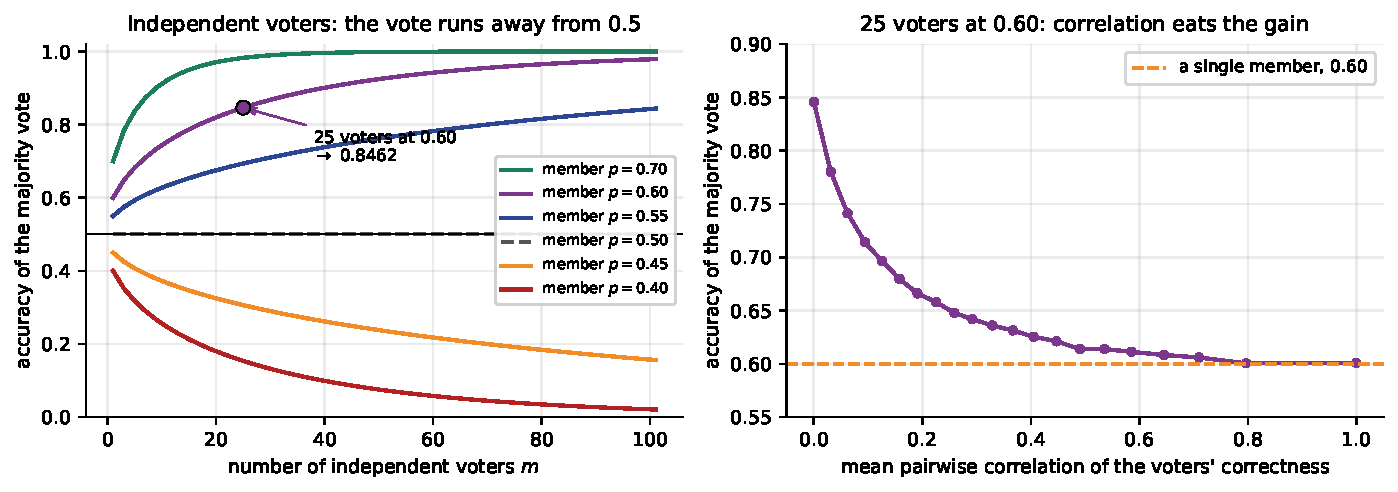
\includegraphics[width=0.98\textwidth]{binomial.pdf}
  \caption{Left: the majority vote of $m$ independent members, for six member
  accuracies. Above $0.5$ the curves run to $1$; below it they run to $0$; at
  $0.5$ nothing happens. Right: the same twenty-five members at $p = 0.60$,
  now correlated. The dashed line is a single member. \textbf{The left panel
  is the advertisement; the right panel is the contract.}}
  \label{fig:binomial}
\end{figure}

\begin{keyidea}
An ensemble helps exactly to the extent that its members \emph{fail on
different rows}. Accuracy of the members is necessary; diversity of the
members is what you are actually buying. Every technique in the rest of these
notes is a way of manufacturing diversity.
\end{keyidea}

\subsection{Ensembles of classifiers: different learners, one vote}

The most obvious way to get diverse members is to use genuinely different
kinds of model. scikit-learn's \texttt{VotingClassifier} does this.

\begin{lstlisting}
from sklearn.ensemble import VotingClassifier
members = [("knn",  make_pipeline(StandardScaler(), KNeighborsClassifier(5))),
           ("tree", DecisionTreeClassifier(max_depth=3, random_state=0)),
           ("lr",   make_pipeline(StandardScaler(),
                                  LogisticRegression(max_iter=5000)))]
for name, mdl in members:
    mdl.fit(Xtr, ytr)
    print("%-5s test accuracy %.4f" % (name, accuracy_score(yte, mdl.predict(Xte))))
vote = VotingClassifier(members, voting="hard").fit(Xtr, ytr)
print("vote  test accuracy %.4f" % accuracy_score(yte, vote.predict(Xte)))
\end{lstlisting}
\begin{codeout}
knn   test accuracy 0.9474
tree  test accuracy 0.9006
lr    test accuracy 0.9591
vote  test accuracy 0.9474
mean pairwise disagreement between members 0.0702
rows where the members were not unanimous  18 of 171
\end{codeout}

\begin{caution}[Report the result you got, not the one you wanted]
The vote scored $0.9474$. Logistic regression alone scored $0.9591$.
\textbf{The ensemble did not beat its best member.} That is a real result and
it is worth more to you than a tidy one.

Three reasons, all visible in the output. Three members is far too few --- go
back to the table in Section~\ref{sec:jury} and notice how slowly $m = 11$
improves on $m = 1$. One member (the depth-3 tree, $0.9006$) is much weaker
than the others and drags a plain unweighted vote down. And most decisively,
on $153$ of the $171$ test rows all three members already agree, so the vote
has only $18$ rows on which it can do anything at all; a single row is
$0.0058$ of the test accuracy here.

The lesson is not that voting does not work. It is that voting needs
\emph{many} members and \emph{comparable} members. Bagging and boosting supply
hundreds of both.
\end{caution}

\subsection{Three ways to manufacture disagreement}

That leaves the design question: how do you produce hundreds of members that
are all decent and all different? There are exactly three knobs, and the rest
of this lecture is one section for each.

\begin{enumerate}[leftmargin=*]
  \item \textbf{Change the rows.} Give each member a different resample of the
    training set. That is \textbf{bagging}, Section~\ref{sec:bag}.
  \item \textbf{Change the columns.} Let each member --- in fact each
    \emph{split} of each member --- see only a random subset of the features.
    Bagging plus this is a \textbf{random forest},
    Section~\ref{sec:rf}.
  \item \textbf{Change the weights.} Make each member concentrate on the rows
    the committee so far gets wrong. That is \textbf{boosting},
    Section~\ref{sec:boost}.
\end{enumerate}

What is \emph{not} on the list: refitting the same deterministic learner on
the same data with a different random seed. That gives $\rho = 1$ and, by the
last row of the copula table, an ensemble worth exactly one member.

\notesources{\AMLUnitVISources}

% =========================================================================
\section{Bagging and the bootstrap}
\label{sec:bag}

\subsection{The bootstrap sample}

A \textbf{bootstrap sample} of a training set of $n$ rows is $n$ rows drawn
\emph{with replacement} from it. Some rows are drawn twice or three times;
some are not drawn at all. Both facts matter. Drawing \emph{without}
replacement would return the training set itself and every member would be
identical; drawing with replacement produces a genuinely different training
set each time, and it is the rows left out that will pay for the free
validation in Section~\ref{sec:oob}.

\begin{worked}[Five rows, four bags]
Take the training set $\{A, B, C, D, E\}$ and draw five rows with replacement,
four times:
\begin{center}
\begin{tabular}{llcl}
  \toprule
  bag & sample & distinct & out-of-bag \\
  \midrule
  1 & E D C B B & 4/5 & $A$ \\
  2 & A A A A E & 2/5 & $B, C, D$ \\
  3 & D E C D E & 3/5 & $A, B$ \\
  4 & D D C C E & 3/5 & $A, B$ \\
  \bottomrule
\end{tabular}
\end{center}
Two things to notice. The four bags are four \emph{different} training sets:
bag 2 is four copies of $A$ and a single $E$, a training set that has never
heard of three of the five rows. And every bag leaves somebody out --- the
model fitted on bag 3 has never seen $A$ or $B$, so predicting $A$ and $B$
with that model is an honest out-of-sample prediction, obtained without
holding anything back.

The distinct fractions here average $3/5 = 0.60$. The next subsection
computes what that average should be.
\end{worked}

\subsection{The $63.2\%$ result, derived}
\label{sec:632}

Fix one particular row. On a single draw the chance of \emph{not} picking it
is $1 - \frac{1}{n}$. The $n$ draws are independent, so
\begin{equation}
  \Pr[\text{row never drawn}] = \Bigl(1 - \frac{1}{n}\Bigr)^{n},
  \qquad
  \Pr[\text{row is in the bag}] = 1 - \Bigl(1 - \frac{1}{n}\Bigr)^{n}.
  \label{eq:632}
\end{equation}
Since $\lim_{n\to\infty}(1 - 1/n)^n = e^{-1} = 0.367879$, the in-bag
probability tends to
\[
  1 - e^{-1} = \mathbf{0.632121}.
\]
By linearity of expectation the \emph{expected fraction} of distinct rows in
a bag is the same number, because each of the $n$ rows is in the bag with that
probability.

\begin{worked}[Check the formula at small $n$]
At $n = 5$: $(1 - 1/5)^5 = 0.8^5 = 0.32768$, so the in-bag fraction is
$0.67232$. The four bags above averaged $0.60$, a little below that, which is
what four draws of a mean-$0.672$ quantity look like --- with only four bags
the sampling error is larger than the gap in either direction.

At $n = 10$: $(0.9)^{10} = 0.348678$, so $0.651322$. Notice how little the
answer moved for a doubling of $n$: the convergence to $0.632121$ is fast
because $(1-1/n)^n = \exp\bigl(n\ln(1 - 1/n)\bigr)
= \exp\bigl(-1 - \frac{1}{2n} - \frac{1}{3n^2} - \cdots\bigr)$, so the error is
$O(1/n)$ and already under $0.004$ by $n = 100$.
\end{worked}

\begin{lstlisting}
rng = np.random.default_rng(0)          # the one seed for this lecture
print("  n     (1-1/n)^n     1-(1-1/n)^n    empirical unique fraction")
for n in (5, 10, 50, 100, 1000, 10000):
    out = (1 - 1 / n) ** n
    emp = np.mean([len(np.unique(rng.integers(0, n, n))) / n
                   for _ in range(2000)])
    print("%6d   %.6f      %.6f       %.6f" % (n, out, 1 - out, emp))
print("limit 1 - 1/e = %.6f" % (1 - np.exp(-1)))
\end{lstlisting}
\begin{codeout}
  n     (1-1/n)^n     1-(1-1/n)^n    empirical unique fraction
     5   0.327680      0.672320       0.674900
    10   0.348678      0.651322       0.655600
    50   0.364170      0.635830       0.637460
   100   0.366032      0.633968       0.634460
  1000   0.367695      0.632305       0.632152
 10000   0.367861      0.632139       0.632156
limit 1 - 1/e = 0.632121
\end{codeout}

Formula and measurement agree to four decimal places from $n = 50$ upwards.
The right-hand panel of Figure~\ref{fig:bootstrap} sharpens the point that
$63.2\%$ is a \emph{mean}: over twenty thousand bootstrap samples of the
$398$-row training split the distinct fraction had mean $0.6325$ and standard
deviation $0.0158$, with individual bags ranging from $0.5704$ to $0.6910$.

\begin{figure}[tb]
  \centering
  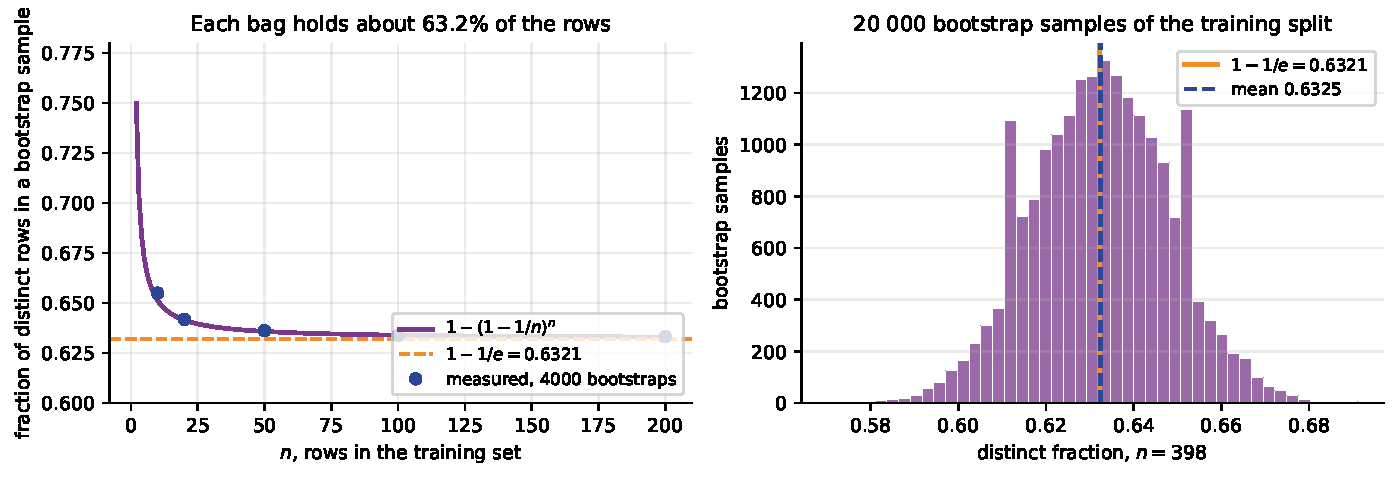
\includegraphics[width=0.98\textwidth]{bootstrap.pdf}
  \caption{Left: the curve $1 - (1-1/n)^n$ against $n$, with the limit
  $1 - 1/e$ and five measured points from four thousand bootstraps each.
  Right: the distribution of the distinct fraction over twenty thousand
  bootstrap samples at $n = 398$. Mean $0.6325$, standard deviation $0.0158$.}
  \label{fig:bootstrap}
\end{figure}

\subsection{The bagging algorithm}

\begin{keyidea}[Bagging]
For $b = 1, \dots, B$: draw a bootstrap sample of the training set and fit a
model $T_b$ on it. Predict by majority vote (classification) or by the mean
(regression) of $T_1, \dots, T_B$.
\end{keyidea}

That is the whole algorithm. Breiman's 1996 paper that introduced it makes the
condition explicit in its abstract: \emph{the vital element is the instability
of the prediction method}. Bagging helps a learner whose output changes a lot
when the training data changes a little. Unpruned decision trees are the
textbook case; ordinary least squares is close to the opposite, and bagging it
buys almost nothing.

\begin{lstlisting}
from sklearn.ensemble import BaggingClassifier
tree = DecisionTreeClassifier(random_state=0).fit(Xtr, ytr)
bag = BaggingClassifier(DecisionTreeClassifier(random_state=0),
                        n_estimators=200, oob_score=True,
                        random_state=0).fit(Xtr, ytr)
print("single unpruned tree   test accuracy %.4f" % tree.score(Xte, yte))
print("bag of 200 such trees  test accuracy %.4f" % bag.score(Xte, yte))
print("bag out-of-bag score                 %.4f" % bag.oob_score_)
\end{lstlisting}
\begin{codeout}
single unpruned tree   test accuracy 0.9064
bag of 200 such trees  test accuracy 0.9298
bag out-of-bag score                 0.9598
OOB minus test                       +0.0300
5-fold CV on the training rows       0.9497
\end{codeout}

Two hundred copies of a learner that scores $0.9064$ score $0.9298$ together:
$+0.0234$, or four test rows, for no change whatsoever to the learner. Same
class, same hyperparameters, same features, same code. The only new thing is
the resampling.

\subsection{Out-of-bag error: validation you did not have to pay for}
\label{sec:oob}

Section~\ref{sec:632} showed that each member misses about $37\%$ of the
training rows. Turn that round: each training row is missed by about $37\%$ of
the members. Those members can be asked to predict it, and their prediction is
a genuine out-of-sample prediction, because that row played no part in
choosing any of their splits.

\begin{keyidea}[Out-of-bag score]
For each training row, aggregate only the members for which that row was
out-of-bag, and score the result against the truth. No rows are held back and
no model is fitted twice.
\end{keyidea}

There is one caveat and you should say it whenever you quote an OOB score:
each OOB prediction comes from a sub-ensemble of roughly $0.37B$ members
rather than all $B$, so for small $B$ the OOB estimate is \emph{pessimistic}
--- it measures a smaller ensemble than the one you will deploy. With $B$ in
the hundreds the effect is far below the noise.

Is it honest in practice? The single split above gave OOB $0.9598$ against a
test score of $0.9298$ --- optimistic by $0.0300$, which looks alarming. One
split proves nothing at all. Repeat over twenty splits.

\begin{lstlisting}
d = []
for s in range(20):
    A, B, a, b = train_test_split(Xb, yb, test_size=0.3, random_state=s,
                                  stratify=yb)
    f = RandomForestClassifier(n_estimators=300, oob_score=True,
                               random_state=s).fit(A, a)
    d.append((f.oob_score_, f.score(B, b)))
d = np.array(d)
print("mean OOB score      %.4f  (sd %.4f)" % (d[:, 0].mean(), d[:, 0].std()))
print("mean held-out score %.4f  (sd %.4f)" % (d[:, 1].mean(), d[:, 1].std()))
print("mean OOB - held-out %+.4f" % (d[:, 0] - d[:, 1]).mean())
print("paired t = %.3f, p = %.3f" % stats.ttest_rel(d[:, 0], d[:, 1]))
\end{lstlisting}
\begin{codeout}
20 random splits of breast_cancer, forest of 300 trees
mean OOB score      0.9584  (sd 0.0054)
mean held-out score 0.9576  (sd 0.0137)
mean OOB - held-out +0.0008
paired t = 0.209, p = 0.836
\end{codeout}

The systematic bias is $+0.0008$, about a seventh of a single test row, and
the paired $t$-test cannot distinguish it from zero ($p = 0.836$). Note also
the standard deviations: $0.0054$ for OOB against $0.0137$ for the held-out
score. The free estimate is not merely unbiased here, it is \emph{less noisy},
because it is computed on all $398$ training rows while the held-out score is
computed on only $171$.

\begin{figure}[tb]
  \centering
  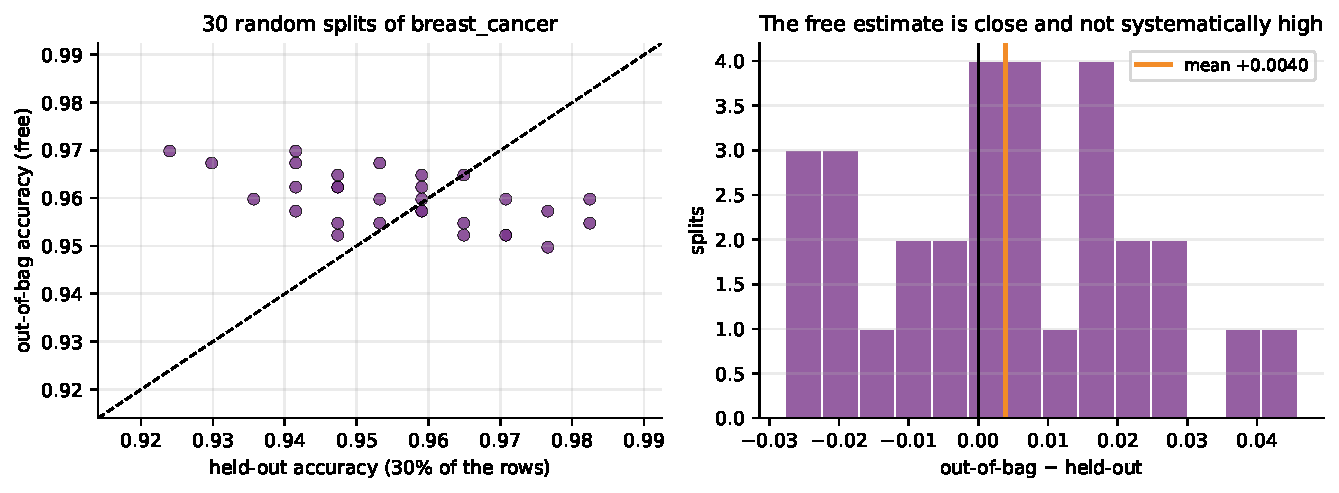
\includegraphics[width=0.92\textwidth]{oob.pdf}
  \caption{Thirty random splits of \texttt{breast\_cancer}, forests of $300$
  trees. Left: OOB accuracy against held-out accuracy, with the line $y = x$.
  Right: the distribution of their difference, centred on
  $+0.0040$ over these thirty splits.}
  \label{fig:oob}
\end{figure}

\begin{caution}[What OOB is and is not]
OOB estimates the \emph{generalisation accuracy of this ensemble}. It is a
legitimate substitute for a validation set --- you may tune
\texttt{max\_features} on it, as Section~\ref{sec:rf} does. It is \emph{not} a
substitute for a final held-out test set if you have tuned on it, for exactly
the reason cross-validation is not: once you select a hyperparameter by
maximising a score, that score is optimistic. And OOB is only available when
\texttt{bootstrap=True}; set \texttt{bootstrap=False} and there is no
out-of-bag anything.
\end{caution}

\notesources{\AMLUnitVISources}

% =========================================================================
\section{Bagging reduces variance, not bias}
\label{sec:var}

\subsection{What averaging can and cannot do}

For squared-error regression, the expected error of a fitted model $\hat f$ at
a point $x$ decomposes exactly:
\begin{equation}
  \mathbb{E}\bigl[(y - \hat f(x))^2\bigr]
    = \underbrace{\bigl(\mathbb{E}[\hat f(x)] - f(x)\bigr)^2}_{\text{bias}^2}
    + \underbrace{\operatorname{Var}[\hat f(x)]}_{\text{variance}}
    + \underbrace{\sigma^2}_{\text{noise}},
  \label{eq:bv}
\end{equation}
where the expectations are over training sets drawn from the same
distribution.

Averaging $B$ models leaves the expectation alone --- the mean of $B$ copies of
a random quantity has the same mean as one copy --- and shrinks the variance.
So bagging can move the second term of \eqref{eq:bv} and nothing else. That is
a prediction, and it is testable.

\subsection{The experiment}

Take $f(x) = \sin(4x) + x$ on $[0, 3]$, draw $120$ training points uniformly
with Gaussian noise of standard deviation $\sigma = 0.35$, and repeat the
whole thing $300$ times. On each of the $300$ training sets fit (a) one
unpruned regression tree and (b) a bag of $50$ of them. Then, at each of $60$
evaluation points, take the mean and the variance of the $300$ predictions.
Because we know $f$ exactly, both terms of \eqref{eq:bv} can be computed
rather than estimated.

\begin{lstlisting}
def truth(x):
    return np.sin(4 * x) + x

xg = np.linspace(0.05, 2.95, 60); fg = truth(xg)
REP, NTR, SD = 300, 120, 0.35

def sweep(make):
    rng = np.random.default_rng(0)
    P = np.zeros((REP, len(xg)))
    for r in range(REP):
        xt = rng.uniform(0, 3, NTR)
        yt = truth(xt) + rng.normal(0, SD, NTR)
        P[r] = make(r).fit(xt[:, None], yt).predict(xg[:, None])
    return P

pt = sweep(lambda r: DecisionTreeRegressor(random_state=r))
pb = sweep(lambda r: BaggingRegressor(DecisionTreeRegressor(random_state=r),
                                      n_estimators=50, random_state=r))
for name, P in (("single deep tree", pt), ("bag of 50 trees", pb)):
    bias2 = np.mean((P.mean(0) - fg) ** 2)
    var = np.mean(P.var(0))
    print("%-16s  bias^2 %.4f   variance %.4f   bias^2+var %.4f"
          % (name, bias2, var, bias2 + var))
\end{lstlisting}
\begin{codeout}
single deep tree  bias^2 0.0005   variance 0.1230   bias^2+var 0.1235
bag of 50 trees   bias^2 0.0002   variance 0.0601   bias^2+var 0.0603
variance fell to 48.8% of the single tree's; bias^2 moved -0.0003
irreducible noise variance 0.1225
\end{codeout}

Variance $0.1230 \to 0.0601$: halved. Bias$^2$ $0.0005 \to 0.0002$: both
numbers are negligible beside the variance, which is the point --- a deep tree
is nearly unbiased to begin with, so there was nothing there for bagging to
fix even if it could. The noise floor $\sigma^2 = 0.35^2 = 0.1225$ is printed
as a reminder that no method can drive the total below it.

\begin{figure}[tb]
  \centering
  
\includegraphics[width=0.99\textwidth]{biasvar.pdf}
  \caption{Left and centre: forty of the three hundred fitted curves, with the
  mean prediction in bold and the true $f(x)$ dashed. The single trees scatter;
  the bagged curves hug the truth. Crucially the two bold lines are in the
  \emph{same place} --- the bias did not move. Right: the two terms of
  \eqref{eq:bv} as bars.}
  \label{fig:biasvar}
\end{figure}

\subsection{The other half of the claim: bag a stump}

Halving a variance that was already the dominant term is a good look for
bagging. To see that it really cannot touch bias, run the identical experiment
with a learner that is \emph{badly} biased: a depth-1 stump, which can produce
only two output values and therefore cannot represent a sine wave at all.

\begin{lstlisting}
ps  = sweep(lambda r: DecisionTreeRegressor(max_depth=1, random_state=r))
pbs = sweep(lambda r: BaggingRegressor(
    DecisionTreeRegressor(max_depth=1, random_state=r),
    n_estimators=50, random_state=r))
\end{lstlisting}
\begin{codeout}
single stump      bias^2 0.1856   variance 0.0281   bias^2+var 0.2137
bag of 50 stumps  bias^2 0.1842   variance 0.0147   bias^2+var 0.1989
bagging removed 48% of the stump's variance and left the bias where it was
\end{codeout}

The variance halves again --- $0.0281 \to 0.0147$, the same $48\%$, which is
reassuring because the mechanism is identical. And the bias moves by
$\mathbf{0.0014}$, less than one percent of itself. Fifty stumps are still a
stump.

\begin{keyidea}
Bagging is a variance reducer and nothing else. Two consequences follow
immediately. \textbf{(1)} Put \emph{deep, unpruned} learners inside a bag ---
you want the high-variance, low-bias end, because variance is what bagging
removes. Pruning the members throws away the wrong half. \textbf{(2)} If your
model is \emph{underfitting}, bagging it will not help. Fixing bias is
boosting's job, which is why boosting exists and why its members are shallow.
\end{keyidea}

\notesources{\AMLUnitVISources}

% =========================================================================
\section{Random forests}
\label{sec:rf}

\subsection{Bagging plus a random subset of features per split}

A \textbf{random forest} is bagging with one extra restriction:

\begin{keyidea}[Random forest]
Grow $B$ trees on $B$ bootstrap samples. At \emph{every split of every tree},
choose \texttt{max\_features} of the $d$ columns at random and search only
those for the best split. Vote.
\end{keyidea}

The default \texttt{max\_features} is $\lfloor\sqrt{d}\rfloor$ for
classification and $d/3$ for regression. For \texttt{breast\_cancer},
$\sqrt{30} = 5.4772$, so scikit-learn's \texttt{'sqrt'} uses $5$ features per
split.

The motivation is Section~\ref{sec:indep}. If one feature is much more
predictive than the others, every bagged tree will put it at the root, and
probably the same feature second as well. The trees then look alike, their
errors correlate, and by the right-hand panel of Figure~\ref{fig:binomial} an
ensemble of near-identical members is worth barely more than one member.
Forbidding the dominant feature at a random $(d - \texttt{max\_features})/d$
of the splits forces those trees to find other structure.

\subsection{Why decorrelation is the only lever left}

Suppose the $B$ members each have variance $\sigma^2$ and every pair has
correlation $\rho$. Then
\begin{equation}
  \operatorname{Var}\Bigl(\frac{1}{B}\sum_{b=1}^{B} T_b\Bigr)
    = \frac{1}{B^2}\Bigl(B\sigma^2 + B(B-1)\rho\sigma^2\Bigr)
    = \rho\,\sigma^2 + \frac{1 - \rho}{B}\,\sigma^2.
  \label{eq:corravg}
\end{equation}

\begin{worked}[Read equation \eqref{eq:corravg} carefully]
The second term has $B$ in the denominator and goes to zero as you add
members. \textbf{The first term does not contain $B$ at all.}

At $B = 100$, as a fraction of one member's variance:
\begin{center}
\begin{tabular}{cc}
  \toprule
  $\rho$ & $\rho + (1-\rho)/B$ \\
  \midrule
  0.00 & 0.0100 \\
  0.10 & 0.1090 \\
  0.30 & 0.3070 \\
  0.50 & 0.5050 \\
  0.80 & 0.8020 \\
  1.00 & 1.0000 \\
  \bottomrule
\end{tabular}
\end{center}
At $\rho = 0.5$, a hundred trees and a million trees are both stuck at
approximately half the variance of one tree. Once $B$ is large the
\emph{only} remaining way to reduce the variance is to reduce $\rho$, and
\texttt{max\_features} is the knob that does it.
\end{worked}

\subsection{Measured: worse trees, better forest}

The prediction is that lowering \texttt{max\_features} lowers both the
correlation between trees \emph{and} the accuracy of each tree, so the
ensemble should be best somewhere in the middle. Measure the correlation as
the mean pairwise Pearson correlation of the members' predicted probabilities
on the test rows.

\begin{lstlisting}
def tree_corr(forest, X):
    """Mean pairwise Pearson correlation of the member trees' P(class 1)."""
    P = np.array([t.predict_proba(X)[:, 1] for t in forest.estimators_])
    C = np.corrcoef(P); k = len(P)
    return (C.sum() - k) / (k * (k - 1))

for label, mf in (("bagging (max_features=30)", None),
                  ("forest  (max_features=5)", "sqrt"),
                  ("forest  (max_features=1)", 1)):
    f = RandomForestClassifier(n_estimators=100, max_features=mf,
                               random_state=0).fit(Xtr, ytr)
    single = np.mean([t.score(Xte, yte) for t in f.estimators_])
    print("%-27s tree corr %.4f   mean single tree %.4f   ensemble %.4f"
          % (label, tree_corr(f, Xte), single, f.score(Xte, yte)))
\end{lstlisting}
\begin{codeout}
bagging (max_features=30)   tree corr 0.8261   mean single tree 0.9130   ensemble 0.9240
forest  (max_features=5)    tree corr 0.7945   mean single tree 0.9110   ensemble 0.9532
forest  (max_features=1)    tree corr 0.7010   mean single tree 0.8861   ensemble 0.9415
\end{codeout}

Exactly as predicted, and it is worth reading the three columns separately.
Correlation falls monotonically, $0.8261 \to 0.7945 \to 0.7010$. Mean member
accuracy falls monotonically too, $0.9130 \to 0.9110 \to 0.8861$. And the
ensemble --- the product of the two competing effects --- peaks in the middle at
$\mathbf{0.9532}$. At \texttt{max\_features=1} the trees have been
decorrelated the most but have become too weak to carry the vote.

Sweeping the whole range confirms the shape and, more usefully, shows that you
can find the optimum without ever touching the test set.

\begin{lstlisting}
for mf in (1, 2, 3, 5, 8, 12, 20, 30):
    f = RandomForestClassifier(n_estimators=200, max_features=mf,
                               oob_score=True, random_state=0).fit(Xtr, ytr)
    single = np.mean([t.score(Xte, yte) for t in f.estimators_])
    print("      %2d         %.4f        %.4f          %.4f   %.4f"
          % (mf, tree_corr(f, Xte), single, f.oob_score_, f.score(Xte, yte)))
\end{lstlisting}
\begin{codeout}
 max_features   tree corr   mean single tree   OOB      test
       1         0.7046        0.8864          0.9673   0.9357
       2         0.7582        0.9030          0.9673   0.9532
       3         0.7698        0.9053          0.9623   0.9474
       5         0.7935        0.9110          0.9698   0.9532
       8         0.8104        0.9135          0.9598   0.9474
      12         0.8132        0.9141          0.9598   0.9532
      20         0.8246        0.9139          0.9598   0.9298
      30         0.8282        0.9135          0.9548   0.9240
\end{codeout}

The OOB column is minimised at \texttt{max\_features=5} --- OOB error $0.0302$,
against $0.0452$ at $30$. That is the scikit-learn default, and it was
selected here using only training rows. The test column is noisier (it is
$171$ rows, so one row is $0.0058$) but tells the same story: everything from
$2$ to $12$ is good, and the plain-bagging end at $30$ is clearly worse.

\begin{figure}[tb]
  \centering
  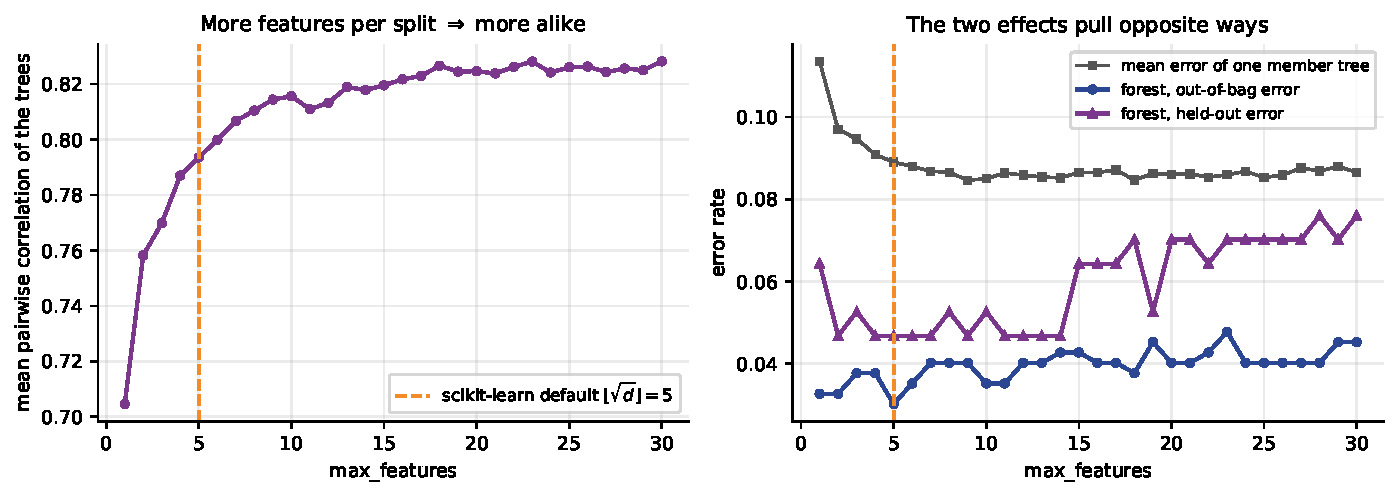
\includegraphics[width=0.98\textwidth]{maxfeatures.pdf}
  \caption{Left: mean pairwise tree correlation rises steadily with
  \texttt{max\_features}. Right: the error of one member falls with
  \texttt{max\_features} while the ensemble error is minimised in the middle.
  Dashed line: the default $\lfloor\sqrt{30}\rfloor = 5$.}
  \label{fig:maxfeatures}
\end{figure}

\subsection{A forest against its own trees}

One last measurement, because it is the whole lecture in five lines.

\begin{lstlisting}
f = RandomForestClassifier(n_estimators=300, oob_score=True,
                           random_state=0).fit(Xtr, ytr)
print("mean over all 300 trees %.4f"
      % np.mean([t.score(Xte, yte) for t in f.estimators_]))
print("worst single tree       %.4f"
      % min(t.score(Xte, yte) for t in f.estimators_))
print("the forest              %.4f" % f.score(Xte, yte))
\end{lstlisting}
\begin{codeout}
a forest is 300 trees; the first three have 13, 16, 18 leaves
their individual test accuracies 0.8889 0.9123 0.8772
mean over all 300 trees          0.9120
worst single tree                0.8480
the forest                       0.9532
\end{codeout}

Not one of the three hundred members is a model you would ship. Each is a
small overfitted tree, grown on $63\%$ of the rows, allowed only five features
per split; the average scores $0.9120$ and the worst scores $0.8480$. The
forest scores $0.9532$, above the average member by $0.0412$ and above every
one of the first three shown. That is Figure~\ref{fig:binomial}'s left panel
happening on real data.

\begin{tryit}[Watch the plateau]
Fit forests with \texttt{n\_estimators} in $\{1, 5, 25, 100, 400\}$ on the
split above and print the test accuracy each time. You should see it rise
steeply and then stop: on the noisy split of Section~\ref{sec:vs} the numbers
were $0.6959$, $0.8012$, $0.9123$, $0.9298$, $0.9298$. \textbf{More trees in a
forest never makes it worse in expectation} --- equation \eqref{eq:corravg}
says the variance of the average is monotone decreasing in $B$ --- it only
makes it slower. On a $171$-row test set expect a jitter of a row or two
either way on top of that. So the honest answer
to ``how many trees'' is ``as many as you can afford, and then stop worrying''.
\end{tryit}

\notesources{\AMLUnitVISources}

% =========================================================================
\section{Feature importance, honestly}
\label{sec:imp}

\subsection{Mean decrease in impurity}

\texttt{RandomForestClassifier.feature\_importances\_} reports the
\textbf{mean decrease in impurity} (MDI). For a single tree, each split
reduces the impurity of the node it acts on; weight that reduction by the
fraction of training rows reaching the node, add up over all splits that used
a given feature, and you have that feature's importance in that tree. Average
over the trees and normalise so the vector sums to $1$.

It is popular because it is free --- the numbers are a by-product of fitting,
requiring no extra data and no extra computation. And it is biased.

\begin{caution}[Impurity importance favours high-cardinality features]
A feature with many distinct values offers many candidate split points. More
candidates means a better \emph{best} candidate, purely by chance, even when
the feature carries no information at all. So MDI systematically scores
high-cardinality columns above low-cardinality ones.

This is the same bias the decision-tree lecture found in information gain,
where a $14$-value \texttt{Day} column scored the maximum possible gain and
built a useless tree. The forest inherits it. scikit-learn's own user guide
states it in as many words: impurity-based importance is ``strongly biased''
and ``favor[s] high cardinality features''.
\end{caution}

\subsection{Demonstration 1: plant three useless columns}

Add to \texttt{breast\_cancer} three columns drawn from a random number
generator: a coin ($2$ values), a die ($6$ values) and a row identifier ($569$
distinct values, a permutation of $0 \dots 568$). None of them has any
relationship to the diagnosis.

\begin{lstlisting}
rng = np.random.default_rng(42); nb = len(Xb)
coin = rng.integers(0, 2, nb).astype(float)    # 2 levels, pure noise
dice = rng.integers(1, 7, nb).astype(float)    # 6 levels, pure noise
uid  = rng.permutation(nb).astype(float)       # 569 levels, pure noise
Xn = np.c_[Xb, coin, dice, uid]
A, B, a, b = train_test_split(Xn, yb, test_size=0.3, random_state=0, stratify=yb)
f = RandomForestClassifier(n_estimators=500, random_state=0).fit(A, a)
imp = f.feature_importances_
\end{lstlisting}
\begin{codeout}
forest test accuracy with the three noise columns added 0.9357
top 5 by impurity importance:
   worst perimeter            0.1404
   worst concave points       0.1200
   mean concave points        0.1161
   worst radius               0.1067
   worst area                 0.0912
the three planted noise columns:
   noise_uid(569)             0.0028   rank 30 of 33
   noise_dice(6)              0.0012   rank 32 of 33
   noise_coin(2)              0.0005   rank 33 of 33
the useless 569-level column scores 5.9 times the useless 2-level column
it outranks 1 of the 30 real clinical measurements
top 3 by permutation importance (held-out rows):
   worst radius               +0.0029
   worst concave points       +0.0023
   worst area                 +0.0010
   noise_uid(569)             +0.0000  (sd 0.0000)
   noise_dice(6)              -0.0006  (sd 0.0018)
   noise_coin(2)              +0.0000  (sd 0.0000)
\end{codeout}

Be precise about what this shows and what it does not. The bias is real and
measurable: the three noise columns rank in exactly cardinality order, and the
$569$-level column scores $5.9$ times the $2$-level column despite both being
the same kind of nothing. But the thirty clinical measurements are genuinely
strong, so the noise still lands at ranks $30$, $32$ and $33$ out of $33$, and
outranks only one real measurement. \textbf{On this dataset the bias distorts
the numbers; it does not mislead you about which columns matter.}

Report that honestly. Then build a case where it does mislead.

\subsection{Demonstration 2: a table where it does mislead}

Eight hundred rows and five columns. \texttt{signal\_binary} takes two values
and agrees with $y$ $75\%$ of the time; that is the only relationship in the
data, so no model can exceed $0.7500$ accuracy. The other four columns --- a
coin, a die, a uniform draw and a permutation --- are pure noise, and the last
two have $800$ distinct values each.

\begin{lstlisting}
rng = np.random.default_rng(0); n = 800
sig = rng.integers(0, 2, n)
ys = np.where(rng.random(n) < 0.25, 1 - sig, sig)     # 75% agreement
Xs = np.c_[sig,                       # 2 levels, informative
           rng.integers(0, 2, n),     # 2 levels, useless
           rng.integers(1, 7, n),     # 6 levels, useless
           rng.random(n),             # 800 levels, useless
           rng.permutation(n)].astype(float)          # 800 levels, useless
A, B, a, b = train_test_split(Xs, ys, test_size=0.3, random_state=0, stratify=ys)
f = RandomForestClassifier(n_estimators=500, random_state=0).fit(A, a)
pi = permutation_importance(f, B, b, n_repeats=30, random_state=0)
\end{lstlisting}
\begin{codeout}
y agrees with signal_binary 75% of the time; nothing else matters
forest test accuracy 0.7333  (the best any model can do is 0.7500)
                     impurity   permutation
signal_binary(2)       0.2715     +0.2136  (sd 0.0294)
noise_coin(2)          0.0237     +0.0083  (sd 0.0115)
noise_dice(6)          0.0829     +0.0189  (sd 0.0131)
noise_cont(800)        0.3110     +0.0081  (sd 0.0145)
noise_uid(800)         0.3109     +0.0114  (sd 0.0127)
impurity importance puts TWO useless columns above the only informative one
useless 800-level column / useless 2-level column = 13.1 times
\end{codeout}

Read the impurity column top to bottom. A uniform random draw scores $0.3110$
and a row identifier scores $0.3109$; the only column carrying any information
scores $0.2715$ and comes \emph{third}. A student who ranked the features by
impurity importance and kept the top two would keep both noise columns and
throw away the signal. Among the four useless columns the ordering is again
pure cardinality: $0.0237$, $0.0829$, $0.3110$, $0.3109$ for $2$, $6$, $800$,
$800$ levels --- a factor of $13.1$ between the two-level and eight-hundred-level
versions of exactly the same nothing.

\subsection{Permutation importance}

\begin{keyidea}[Permutation importance]
Score the fitted model on \textbf{held-out} rows. Randomly shuffle one column,
destroying its relationship with $y$ while leaving its marginal distribution
alone, and score again. The drop is that column's importance. Repeat several
times and average.
\end{keyidea}

It cannot be fooled by cardinality because it never looks at the tree
structure. It asks only the question you actually care about: \emph{if this
column were destroyed, would the predictions get worse?} Shuffling a row
identifier changes nothing the model depends on, so the score does not fall
and the importance is about zero.

The right-hand columns of the output above are exactly that measurement, with
thirty repeats. \texttt{signal\_binary} scores $\mathbf{+0.2136}$ against
$+0.0081$ and $+0.0114$ for the two $800$-level noise columns --- a separation
of about $19\times$, in the correct direction, with standard deviations small
enough ($0.0294$ against $0.0145$) that the ordering is not an accident.

\begin{figure}[tb]
  \centering
  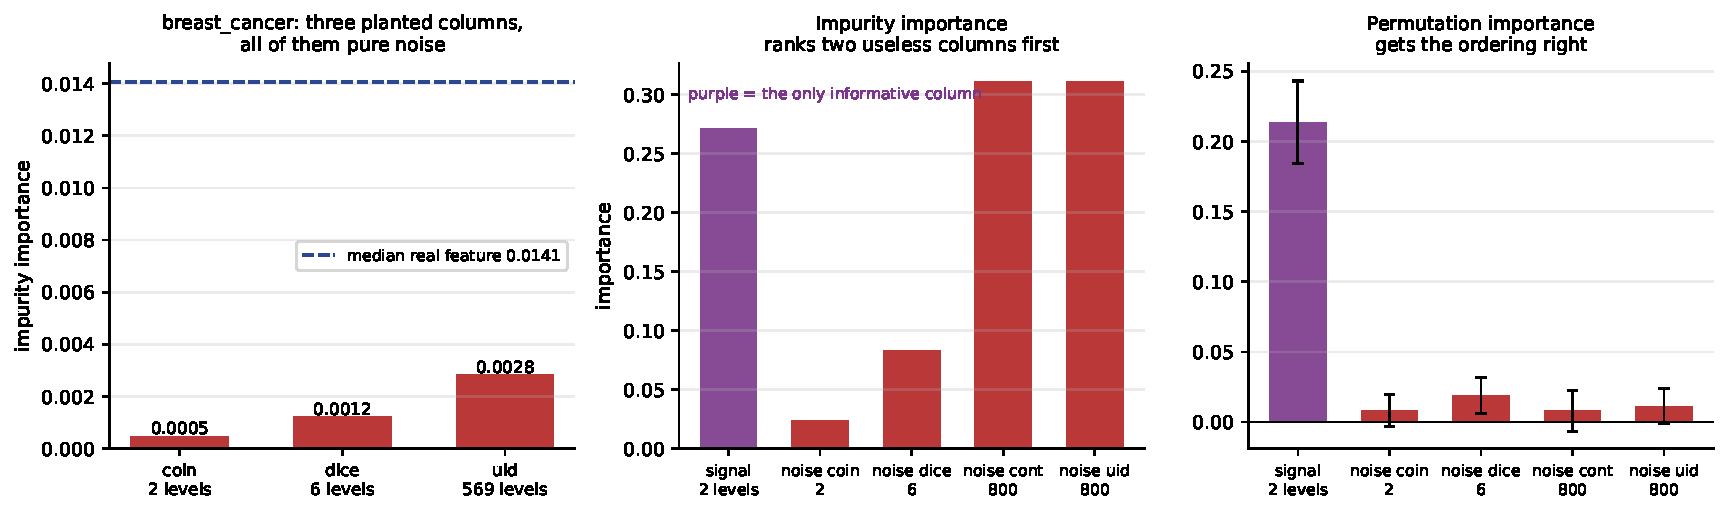
\includegraphics[width=0.99\textwidth]{importance.pdf}
  \caption{Left: on \texttt{breast\_cancer}, the impurity importance of the
  three planted columns rises with cardinality although all three are pure
  noise; the dashed line is the median real feature. Centre and right: on the
  designed table, impurity puts two noise columns above the informative one
  and permutation importance does not. Red is noise in every panel.}
  \label{fig:importance}
\end{figure}

\begin{caution}[Two things permutation importance still cannot do]
\textbf{Compute it on held-out rows.} On training rows an overfitted model
depends heavily on columns that do not generalise, and you will measure the
overfitting rather than the signal.

\textbf{Beware correlated features.} If two columns carry the same
information, shuffling either one leaves the model able to read the other, so
both score near zero and both look useless. On \texttt{breast\_cancer}, whose
thirty features are strongly intercorrelated (\texttt{worst radius},
\texttt{worst perimeter} and \texttt{worst area} are nearly the same
measurement), this is exactly why the permutation importances in
Demonstration~1 are so small --- $+0.0029$ for the best feature. That is a
real limitation, not a bug, and the usual remedy is to cluster correlated
features and permute a cluster at a time.
\end{caution}

\notesources{\AMLUnitVISources}

% =========================================================================
\section{Boosting}
\label{sec:boost}

\subsection{Boosting inverts every design decision in bagging}

Bagging trains its members in parallel, on resampled rows, deep, and gives
them an equal vote. Boosting trains them in sequence, on reweighted rows,
shallow, and gives them a weighted vote. The reason for every one of those
inversions is the same: boosting attacks \textbf{bias}, which is the half of
equation \eqref{eq:bv} that bagging cannot reach.

\begin{keyidea}[Boosting]
Fit a weak learner. Increase the weight of the rows it got wrong. Fit another
weak learner on the reweighted data. Repeat. Predict with a weighted vote in
which better members count for more.
\end{keyidea}

Because each new member is trained specifically on what the committee still
gets wrong, a boosted ensemble of stumps --- models far too simple to fit
anything on their own --- can drive training error to zero. Section~\ref{sec:adahand}
shows that happening on ten points.

\subsection{The AdaBoost algorithm}

Labels are $y_i \in \{-1, +1\}$. Initialise $w_i = 1/n$ for all $n$ training
rows. For $t = 1, \dots, T$:

\begin{enumerate}[leftmargin=*]
  \item Fit a weak learner $h_t$ to the training data weighted by $w$.
  \item Compute the weighted error
    $\displaystyle \varepsilon_t = \sum_{i \,:\, h_t(x_i) \neq y_i} w_i$.
  \item Compute the member weight
    \begin{equation}
      \alpha_t = \frac{1}{2}\ln\frac{1 - \varepsilon_t}{\varepsilon_t}.
      \label{eq:alpha}
    \end{equation}
  \item Reweight and renormalise:
    \begin{equation}
      w_i \leftarrow \frac{w_i\,e^{-\alpha_t y_i h_t(x_i)}}{Z_t},
      \qquad
      Z_t = \sum_j w_j\,e^{-\alpha_t y_j h_t(x_j)}.
      \label{eq:reweight}
    \end{equation}
\end{enumerate}
Predict with $\operatorname{sign} F(x)$ where
$F(x) = \sum_{t=1}^{T}\alpha_t h_t(x)$.

Two things to read carefully. In \eqref{eq:alpha}, $\alpha_t$ is large when
$\varepsilon_t$ is small: a member that solved a hard weighted problem is
trusted more. It is exactly zero at $\varepsilon_t = 0.5$ (a member no better
than chance gets no vote) and negative below that, which is the algorithm
correctly deciding to use a worse-than-chance member backwards.

In \eqref{eq:reweight}, the product $y_i h_t(x_i)$ is $+1$ when the member is
right and $-1$ when it is wrong, so the multiplier is $e^{-\alpha_t} < 1$ for
correct rows and $e^{+\alpha_t} > 1$ for incorrect ones. One expression does
both jobs, and $Z_t$ puts the weights back on the simplex.

\subsection{Three rounds by hand}
\label{sec:adahand}

Ten points on a line: $x = 0, 1, \dots, 9$ with labels
\[
  y = +1,\ +1,\ +1,\ -1,\ -1,\ -1,\ +1,\ +1,\ +1,\ -1.
\]
The weak learner is a decision stump: pick a threshold $\theta$ and a polarity
$s \in \{+1, -1\}$, and predict $s$ when $x < \theta$ and $-s$ otherwise. No
single stump can classify these ten points, because the labels change sign
three times and a stump changes sign once.

\begin{worked}[Round 1]
All weights are $w_i = 0.1$. Search every threshold and both polarities and
count weighted errors. The best is $\theta = 2.5$, $s = +1$: predict $+1$ for
$x \in \{0,1,2\}$ and $-1$ for $x \in \{3,\dots,9\}$. That is right on
$0,1,2$ (label $+1$), right on $3,4,5,9$ (label $-1$), and wrong on
$6,7,8$ (label $+1$, predicted $-1$). Three wrong rows, each of weight $0.1$:
\[
  \varepsilon_1 = 0.1 + 0.1 + 0.1 = \mathbf{0.3000}.
\]
Then
\[
  \alpha_1 = \tfrac12 \ln\frac{1 - 0.3}{0.3}
           = \tfrac12 \ln 2.33333
           = \tfrac12 (0.847298)
           = \mathbf{0.423649}.
\]
Reweight. Wrong rows are multiplied by $e^{+0.423649} = 1.527525$, giving
$0.1 \times 1.527525 = 0.152753$ each. Right rows are multiplied by
$e^{-0.423649} = 0.654654$, giving $0.065465$ each. The normaliser is
\[
  Z_1 = 3(0.152753) + 7(0.065465) = 0.458258 + 0.458258 = 0.916515.
\]
(That the two halves come out equal is not a coincidence: AdaBoost's $\alpha$
is chosen precisely so that after reweighting the misclassified rows carry
total weight exactly $0.5$.) Dividing,
\[
  w_{6,7,8} = \frac{0.152753}{0.916515} = \mathbf{0.1667},
  \qquad
  w_{\text{others}} = \frac{0.065465}{0.916515} = \mathbf{0.0714}.
\]
Check: $3(0.1667) + 7(0.0714) = 0.5001 + 0.4998 = 0.9999 \approx 1$. Good.
\end{worked}

\begin{worked}[Rounds 2 and 3]
\textbf{Round 2} starts with $6, 7, 8$ heavy at $0.1667$ and everything else at
$0.0714$. The best stump is now $\theta = 8.5$, $s = +1$: predict $+1$ for
$x < 8.5$ and $-1$ for $x = 9$. It gets $0,1,2$ right, $6,7,8$ right (which is
what the heavy weights were pushing for), $9$ right, and $3,4,5$ wrong. Those
three now carry $0.0714$ each:
\[
  \varepsilon_2 = 3(0.0714) = \mathbf{0.2143},
  \qquad
  \alpha_2 = \tfrac12 \ln\frac{0.7857}{0.2143} = \mathbf{0.649642}.
\]
Reweighting makes $3, 4, 5$ the heavy rows at $0.1667$, drops $6,7,8$ to
$0.1061$ and $0,1,2,9$ to $0.0455$.

\textbf{Round 3} therefore arrives with $3, 4, 5$ heavy, and the best stump
\emph{flips polarity}: $\theta = 5.5$, $s = -1$, predicting $-1$ for $x < 5.5$
and $+1$ for $x \geq 5.5$. It gets $3,4,5$ right and $6,7,8$ right, and is
wrong on $0,1,2$ (weight $0.0455$ each) and $9$ (weight $0.0455$):
\[
  \varepsilon_3 = 4(0.0455) = \mathbf{0.1818},
  \qquad
  \alpha_3 = \tfrac12 \ln\frac{0.8182}{0.1818} = \mathbf{0.752039}.
\]

The pattern to take away: $\varepsilon$ falls, $0.3000 \to 0.2143 \to 0.1818$,
and $\alpha$ rises, $0.4236 \to 0.6496 \to 0.7520$. Each round faces a harder
weighted problem than the last and is trusted more for solving it.
\end{worked}

\begin{lstlisting}
def best_stump(x, y, w):
    best = None
    for t in np.arange(-0.5, 10, 1.0):
        for s in (+1, -1):
            h = np.where(x < t, s, -s).astype(float)
            err = w[h != y].sum()
            if best is None or err < best[0] - 1e-12:
                best = (err, t, s, h)
    return best

x = np.arange(10).astype(float)
y = np.array([1, 1, 1, -1, -1, -1, 1, 1, 1, -1]).astype(float)
w = np.full(10, 0.1)
alphas, hs = [], []
for rnd in range(1, 4):
    err, t, s, h = best_stump(x, y, w)
    alpha = 0.5 * np.log((1 - err) / err)
    alphas.append(alpha); hs.append(h)
    w = w * np.exp(-alpha * y * h); w = w / w.sum()
\end{lstlisting}
\begin{codeout}
round 1: stump  h(x) = +1 if x < 2.5 else -1
   weighted error  eps = 0.3000
   alpha = 0.5*ln((1-eps)/eps) = 0.4236
   misclassified points x = 6, 7, 8
   new weights 0.0714 0.0714 0.0714 0.0714 0.0714 0.0714 0.1667 0.1667 0.1667 0.0714
   sign(F) so far gets 7 of 10 right
round 2: stump  h(x) = +1 if x < 8.5 else -1
   weighted error  eps = 0.2143
   alpha = 0.5*ln((1-eps)/eps) = 0.6496
   misclassified points x = 3, 4, 5
   new weights 0.0455 0.0455 0.0455 0.1667 0.1667 0.1667 0.1061 0.1061 0.1061 0.0455
   sign(F) so far gets 7 of 10 right
round 3: stump  h(x) = -1 if x < 5.5 else +1
   weighted error  eps = 0.1818
   alpha = 0.5*ln((1-eps)/eps) = 0.7520
   misclassified points x = 0, 1, 2, 9
   new weights 0.1250 0.1250 0.1250 0.1019 0.1019 0.1019 0.0648 0.0648 0.0648 0.1250
   sign(F) so far gets 10 of 10 right
\end{codeout}

\subsection{The combined classifier}

Now assemble $F(x) = 0.4236\,h_1(x) + 0.6496\,h_2(x) + 0.7520\,h_3(x)$.

\begin{codeout}
 x      f1      f2      f3       F(x)   sign  y
 0  +1.0000 +1.0000 -1.0000  +0.3213    +1   +1
 1  +1.0000 +1.0000 -1.0000  +0.3213    +1   +1
 2  +1.0000 +1.0000 -1.0000  +0.3213    +1   +1
 3  -1.0000 +1.0000 -1.0000  -0.5260    -1   -1
 4  -1.0000 +1.0000 -1.0000  -0.5260    -1   -1
 5  -1.0000 +1.0000 -1.0000  -0.5260    -1   -1
 6  -1.0000 +1.0000 +1.0000  +0.9780    +1   +1
 7  -1.0000 +1.0000 +1.0000  +0.9780    +1   +1
 8  -1.0000 +1.0000 +1.0000  +0.9780    +1   +1
 9  -1.0000 -1.0000 +1.0000  -0.3213    -1   -1
training errors of the 3-round ensemble: 0
training errors of the best single stump: 3
\end{codeout}

Check two rows with a pen. At $x = 0$:
$+0.4236 + 0.6496 - 0.7520 = +0.3212$, positive, so class $+1$, which is
right. At $x = 6$: $-0.4236 + 0.6496 + 0.7520 = +0.9780$, positive, class
$+1$, right. Look down the $f_1$, $f_2$, $f_3$ columns: not one of them
matches the $y$ column, and each of the three individually gets at least three
points wrong. Their weighted sum gets all ten.

\begin{figure}[tb]
  \centering
  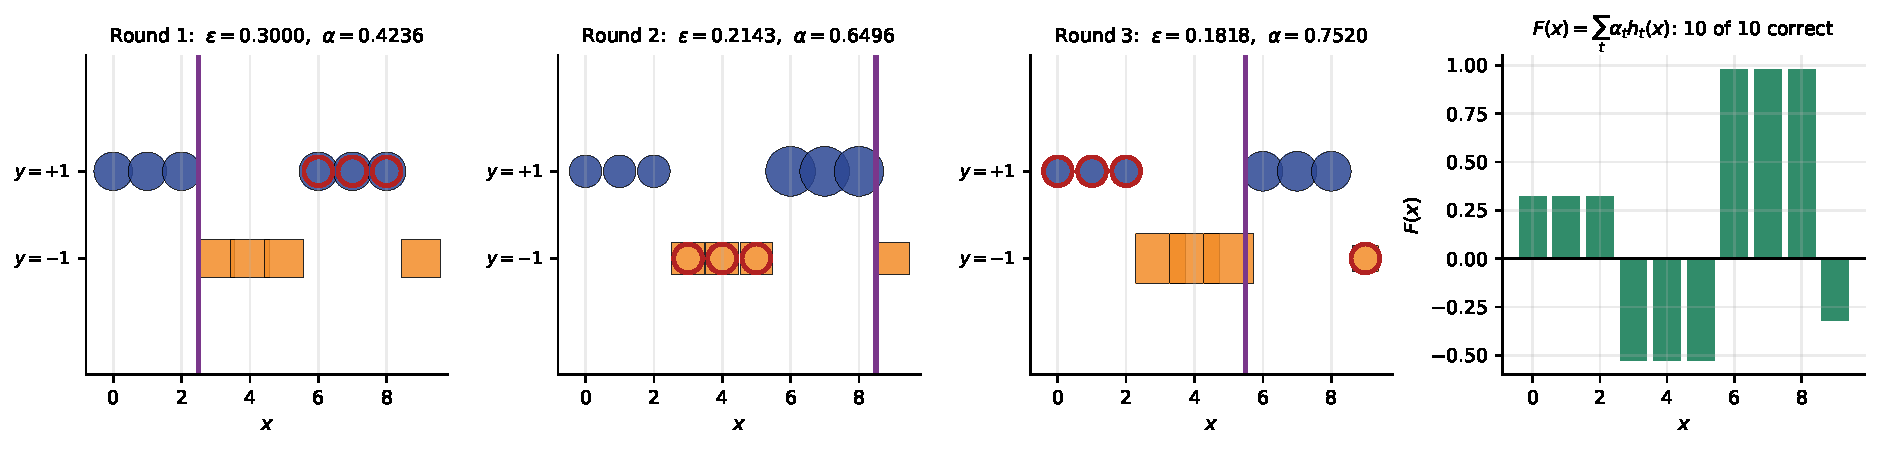
\includegraphics[width=0.99\textwidth]{adaboost.pdf}
  \caption{Three rounds of AdaBoost. Marker area is the row's current weight;
  the vertical line is the stump's threshold; red circles are that round's
  mistakes --- and they are exactly the markers that grow in the next panel.
  Right: $F(x)$, green where its sign matches $y$.}
  \label{fig:adaboost}
\end{figure}

\subsection{The same thing from \texttt{AdaBoostClassifier}}

\begin{lstlisting}
from sklearn.ensemble import AdaBoostClassifier
ada = AdaBoostClassifier(DecisionTreeClassifier(max_depth=1, random_state=0),
                         n_estimators=3, random_state=0).fit(x[:, None], y)
print("sklearn estimator_errors_  ", ada.estimator_errors_)
print("sklearn estimator_weights_ ", ada.estimator_weights_)
\end{lstlisting}
\begin{codeout}
sklearn estimator_errors_  0.3000 0.2143 0.1818
hand-computed eps          0.3000 0.2143 0.1818
sklearn estimator_weights_ 0.8473 1.2993 1.5041
hand-computed alpha        0.4236 0.6496 0.7520
ratio sklearn/hand         2.0000 2.0000 2.0000
sklearn training errors 0, stump thresholds [2.5, 8.5, 5.5]
\end{codeout}

Every weighted error matches to four decimals and all three thresholds match
exactly --- $2.5$, $8.5$, $5.5$, the same stumps in the same order. The member
weights differ by \textbf{exactly a factor of two, every time}, and that is
not a discrepancy to be explained away.

scikit-learn implements SAMME, the multiclass generalisation of AdaBoost,
whose member weight is
\[
  \alpha_t^{\text{SAMME}}
    = \ln\frac{1 - \varepsilon_t}{\varepsilon_t} + \ln(K - 1)
\]
for $K$ classes. With $K = 2$ the second term is $\ln 1 = 0$ and the first is
$2\alpha_t$. Multiplying every member weight by the same positive constant
cannot change $\operatorname{sign}\sum_t \alpha_t h_t(x)$, so the two
ensembles make identical predictions --- both get all ten right.

\subsection{Gradient boosting: fit the residuals}

AdaBoost reweights rows because for classification that is what ``pay more
attention to this row'' means. For squared-error regression there is a more
direct move: fit the next member to \textbf{what is left over}.

\begin{keyidea}[Gradient boosting, squared error]
Start with $F_0(x) = \bar y$. For $m = 1, 2, \dots$: compute the residuals
$r_i = y_i - F_{m-1}(x_i)$, fit a small tree $g_m$ to $(x_i, r_i)$, and set
$F_m = F_{m-1} + \eta\,g_m$.
\end{keyidea}

The name comes from the observation that for squared-error loss
$L = \tfrac12\sum_i (y_i - F(x_i))^2$, the negative gradient with respect to
the prediction at row $i$ is $-\partial L / \partial F(x_i) = y_i - F(x_i)$,
which \emph{is} the residual. Boosting is therefore gradient descent carried
out in the space of functions, one small tree per step, and other loss
functions give other pseudo-residuals.

\begin{worked}[Three stages on eight points]
Take $x = 1, \dots, 8$ and $y = 5, 5, 6, 6, 9, 9, 10, 10$, with $\eta = 1$ and
depth-1 stumps.

$F_0 = \bar y = 7.5$. The residuals are $-2.5, -2.5, -1.5, -1.5, +1.5, +1.5,
+2.5, +2.5$ and the initial $\mathrm{SSE} = 4(2.5^2) + 4(1.5^2)$ --- no,
count them properly: $2(2.5^2) + 2(1.5^2) + 2(1.5^2) + 2(2.5^2)
= 12.5 + 4.5 + 4.5 + 12.5 = 34$.

\textbf{Stage 1.} The best depth-1 split of those residuals is at $x < 4.5$;
the left leaf holds $-2.5, -2.5, -1.5, -1.5$ with mean $-2.0$ and the right
leaf holds $+1.5, +1.5, +2.5, +2.5$ with mean $+2.0$. So
$F_1 = 5.5, 5.5, 5.5, 5.5, 9.5, 9.5, 9.5, 9.5$ and
$\mathrm{SSE} = 4(0.5^2) + 4(0.5^2) = 2.0$.

\textbf{Stage 2.} The new residuals are $-0.5, -0.5, +0.5, +0.5, -0.5, -0.5,
+0.5, +0.5$. The best split is $x < 2.5$: left mean $-0.5$, right mean
$(0.5 + 0.5 - 0.5 - 0.5 + 0.5 + 0.5)/6 = 0.1\overline{6}$. So
$F_2 = 5.0, 5.0, 5.667, 5.667, 9.667, 9.667, 9.667, 9.667$ and
$\mathrm{SSE} = 1.3333$.

\textbf{Stage 3.} Split at $x < 6.5$ gives $F_3 = 4.889, 4.889, 5.556, 5.556,
9.556, 9.556, 10.000, 10.000$ and $\mathrm{SSE} = 1.0370$.
\end{worked}

\begin{lstlisting}
xr = np.arange(1, 9).astype(float)
yr = np.array([5.0, 5.0, 6.0, 6.0, 9.0, 9.0, 10.0, 10.0])
Fm = np.full(8, yr.mean())
for m in range(1, 4):
    r = yr - Fm
    st = DecisionTreeRegressor(max_depth=1, random_state=0).fit(xr[:, None], r)
    Fm = Fm + st.predict(xr[:, None])
    print("   SSE %.4f" % np.sum((yr - Fm) ** 2))
\end{lstlisting}
\begin{codeout}
stage 0: F0 = mean(y) = 7.5000
   residuals -2.500 -2.500 -1.500 -1.500 +1.500 +1.500 +2.500 +2.500
stage 1: stump on the residuals, split at x < 4.5
   stump output -2.000 -2.000 -2.000 -2.000 +2.000 +2.000 +2.000 +2.000
   F1           +5.500 +5.500 +5.500 +5.500 +9.500 +9.500 +9.500 +9.500
   SSE 2.0000
stage 2: stump on the residuals, split at x < 2.5
   stump output -0.500 -0.500 +0.167 +0.167 +0.167 +0.167 +0.167 +0.167
   F2           +5.000 +5.000 +5.667 +5.667 +9.667 +9.667 +9.667 +9.667
   SSE 1.3333
stage 3: stump on the residuals, split at x < 6.5
   stump output -0.111 -0.111 -0.111 -0.111 -0.111 -0.111 +0.333 +0.333
   F3           +4.889 +4.889 +5.556 +5.556 +9.556 +9.556 +10.000 +10.000
   SSE 1.0370
\end{codeout}

\begin{lstlisting}
from sklearn.ensemble import GradientBoostingRegressor
gbm = GradientBoostingRegressor(n_estimators=3, learning_rate=1.0,
                                max_depth=1, random_state=0).fit(xr[:, None], yr)
print("max abs difference  %.2e" % np.max(np.abs(gbm.predict(xr[:, None]) - Fm)))
\end{lstlisting}
\begin{codeout}
sklearn init_.constant_  7.5000   (hand: mean = 7.5000)
sklearn predictions +4.889 +4.889 +5.556 +5.556 +9.556 +9.556 +10.000 +10.000
hand F3             +4.889 +4.889 +5.556 +5.556 +9.556 +9.556 +10.000 +10.000
max abs difference  0.00e+00
\end{codeout}

Not approximately equal --- \emph{bit-for-bit} identical. The library's
initial constant is the mean, and its three stages are the three stumps you
just fitted by hand.

\begin{figure}[tb]
  \centering
  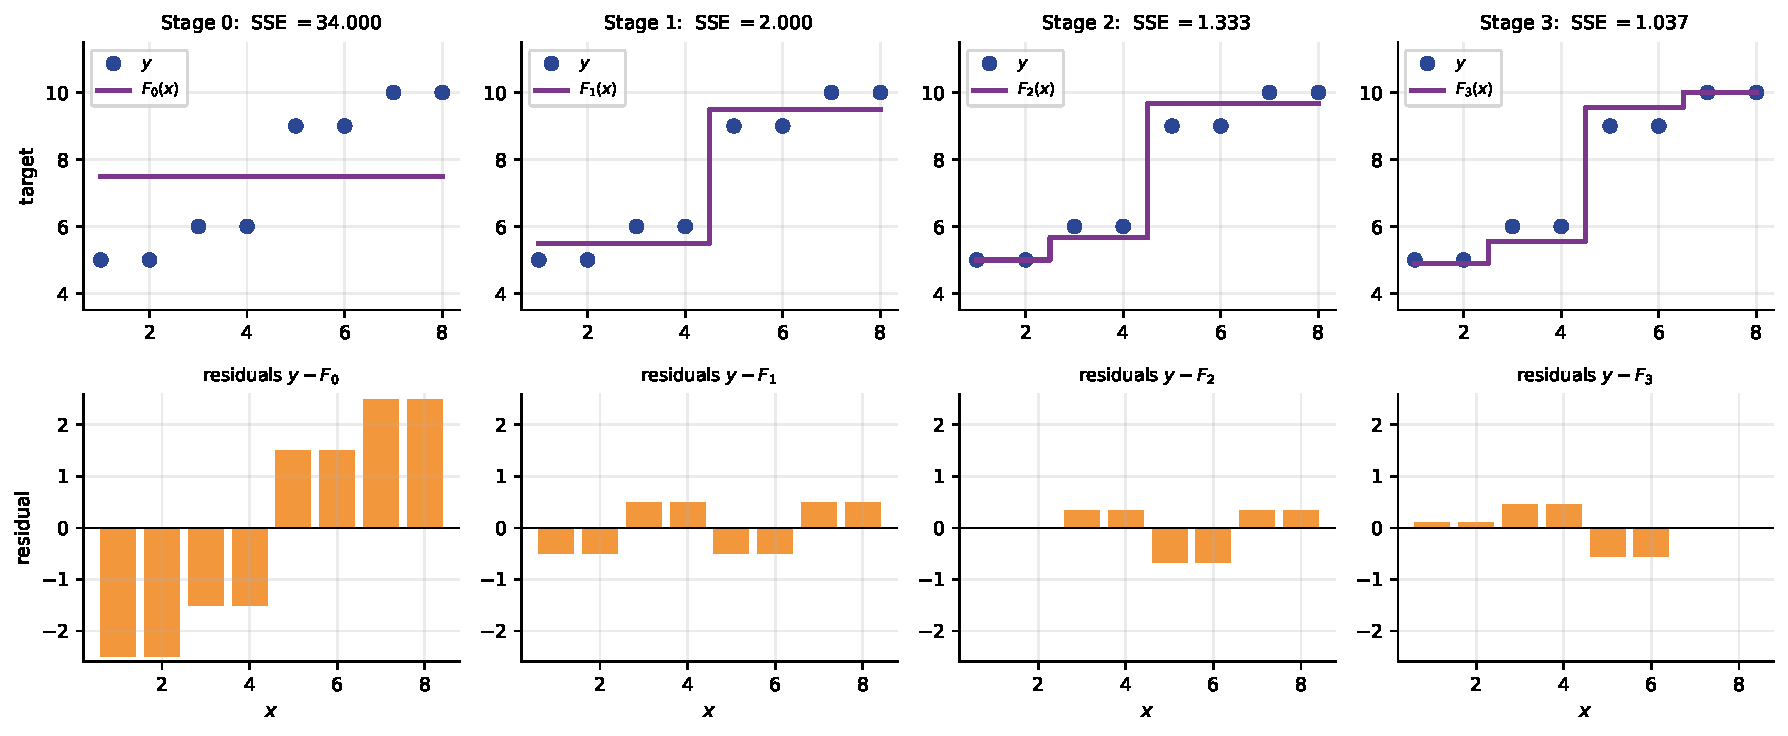
\includegraphics[width=0.97\textwidth]{gradboost.pdf}
  \caption{Gradient boosting on eight points. Top: the staircase $F_m$ closing
  on the data, with the sum of squared errors in each title. Bottom: the
  residuals $y - F_m$ that the next stump will be fitted to.}
  \label{fig:gradboost}
\end{figure}

\begin{caution}[The learning rate]
$\eta$ was set to $1.0$ above so that the hand computation and the library
would agree exactly. \textbf{Do not use $\eta = 1$ in practice.} The default
is $0.1$ and $0.05$ is common: add a small multiple of each stump, and use
many more of them. Small steps generalise better than a few large ones, and
$\eta$ and \texttt{n\_estimators} trade off against each other --- halving
$\eta$ roughly doubles the number of stages you need. Unlike a forest, where
more trees is always safe, \texttt{n\_estimators} is a real hyperparameter
here, and Section~\ref{sec:vs} shows what happens if you get it wrong.
\end{caution}

\notesources{\AMLUnitVISources}

% =========================================================================
\section{Bagging against boosting}
\label{sec:vs}

\subsection{The comparison}

\begin{center}
\small
\begin{tabular}{lll}
  \toprule
   & \textbf{Bagging / random forests} & \textbf{Boosting} \\
  \midrule
  Members trained & in parallel, independently & in sequence, on the last's
    errors \\
  Data each member sees & a bootstrap resample & the same rows, reweighted \\
  Member depth & deep, unpruned & shallow: stumps or depth 2--3 \\
  Aggregation & equal vote & weighted by $\alpha_t$ \\
  Attacks & \textbf{variance} & \textbf{bias} \\
  More members & plateaus; safe & can overfit; must be watched \\
  Label noise & robust: averages it away & \textbf{fragile}: chases it \\
  Parallelisable & yes, trivially & no, inherently sequential \\
  Tuning needed & almost none & $\eta$, depth, $T$ \\
  Free validation & yes (\texttt{oob\_score\_}) & no \\
  \bottomrule
\end{tabular}
\end{center}

The row that matters most in practice is label noise. A mislabelled training
row is a row that every reasonable member gets wrong --- which is precisely the
signal AdaBoost uses to decide a row deserves more weight. Boosting will keep
increasing that row's weight until the ensemble is partly built around it.
Bagging has no such mechanism; the mislabelled row is one vote among $n$ in
each bag and is averaged away.

\subsection{Demonstrated: flip the training labels}

Flip a fraction of the \emph{training} labels at random, leave the test labels
clean, and average over ten splits.

\begin{lstlisting}
for frac in (0.00, 0.10, 0.20, 0.30, 0.40):
    accs = []
    for s in range(10):                    # splits 0..9: the sweep is derived
        A, B, a, b = train_test_split(Xb, yb, test_size=0.3, random_state=s,
                                      stratify=yb)   # from the lecture seed 0
        rr = np.random.default_rng(1000 + s)   # flip stream, clear of the split
        a2 = a.copy()
        k = int(round(frac * len(a2)))
        if k:
            fl = rr.choice(len(a2), k, replace=False)
            a2[fl] = 1 - a2[fl]
        rf = RandomForestClassifier(n_estimators=200, random_state=s).fit(A, a2)
        ab = AdaBoostClassifier(DecisionTreeClassifier(max_depth=1,
                                random_state=s),
                                n_estimators=200, random_state=s).fit(A, a2)
        dt = DecisionTreeClassifier(random_state=s).fit(A, a2)
        accs.append((rf.score(B, b), ab.score(B, b), dt.score(B, b)))
    print(" %3d%%        %.4f              %.4f            %.4f"
          % (int(frac * 100), *np.mean(accs, axis=0)))
\end{lstlisting}
\begin{codeout}
noise   RandomForest(200)   AdaBoost(200 stumps)   single tree
   0%        0.9596              0.9684            0.9322
  10%        0.9503              0.9129            0.8298
  20%        0.9368              0.8789            0.7415
  30%        0.8871              0.8240            0.6661
  40%        0.7327              0.6725            0.5637
\end{codeout}

Say the first line before you say anything else: \textbf{at $0\%$ noise
AdaBoost is better}, by $0.0088$. On clean data, boosting is usually the
stronger method, and a lecture that only showed the noisy columns would be
teaching you a false generalisation.

Then follow the columns down. By $10\%$ noise the forest is ahead by $0.0374$,
by $20\%$ by $0.0579$, and by $40\%$ by $0.0602$. The crossover happens almost
immediately, somewhere below $10\%$ --- which is well inside the range of label
error you should expect in real hand-annotated data.

Note also the third column. The single unpruned tree collapses fastest of all,
from $0.9322$ to $0.5637$, barely above chance. Both ensembles beat it
everywhere by a wide margin. The argument of this section is forest versus
boosting; the argument of the whole lecture is ensemble versus not.

\begin{figure}[tb]
  \centering
  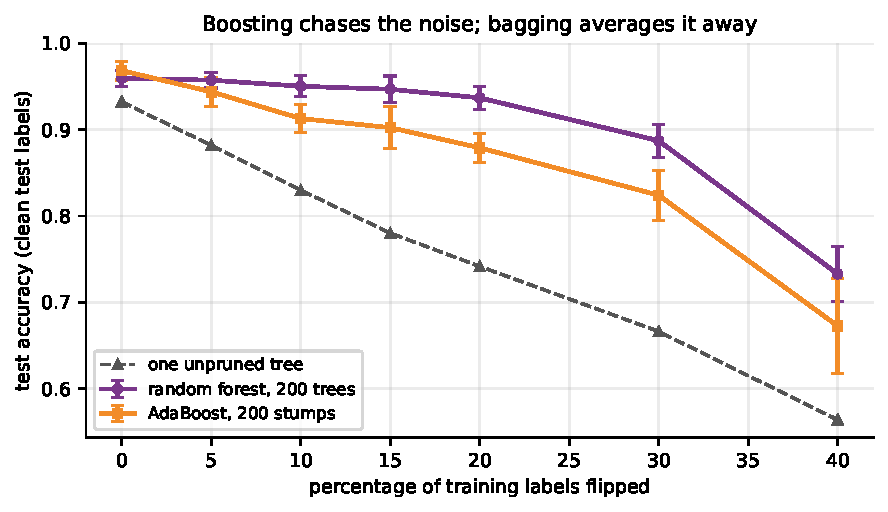
\includegraphics[width=0.72\textwidth]{noise.pdf}
  \caption{Test accuracy on clean labels against the percentage of training
  labels flipped, averaged over ten splits with error bars at one standard
  deviation. AdaBoost starts higher and crosses below the forest almost
  immediately.}
  \label{fig:noise}
\end{figure}

\subsection{How many estimators?}

The second practical difference is what happens as $T$ grows. Take one split,
flip $25\%$ of its training labels, and track both methods stage by stage.
Both the split and the flips come from the lecture's one seed:

\begin{lstlisting}
A, B, a, b = train_test_split(Xb, yb, test_size=0.3, random_state=0,
                              stratify=yb)
rr = np.random.default_rng(0)              # the one seed for this lecture
a2 = a.copy()
fl = rr.choice(len(a2), int(0.25 * len(a2)), replace=False)
a2[fl] = 1 - a2[fl]                        # flip a quarter of the labels
\end{lstlisting}
\begin{codeout}
25% of the training labels flipped
  trees     forest test acc   AdaBoost test acc
     1         0.6959            0.9006
     5         0.8012            0.9006
    10         0.8129            0.9006
    25         0.9123            0.9064
    50         0.9298            0.8480
   100         0.9298            0.8480
   200         0.9298            0.8129
   400         0.9298            0.8070
   800         0.9240            0.7719
forest:   best 0.9298 at T=50, final 0.9240, drop from peak -0.0058
AdaBoost: best 0.9064 at T=19, final 0.7719, drop from peak -0.1345
AdaBoost training accuracy at T=800: 0.9648
\end{codeout}

The forest climbs and flattens. Between $T = 50$ and $T = 800$ it moves by
$0.0058$, which on $171$ test rows is exactly one row --- noise. AdaBoost peaks
at $T = 19$ with $0.9064$ and then loses $\mathbf{0.1345}$ over the remaining
seven hundred and eighty-one rounds, ending far below where it started at
$T = 1$.

The last line explains why. At $T = 800$ AdaBoost's \emph{training} accuracy is
$0.9648$ on labels that are $25\%$ wrong. It has memorised the flipped labels,
which is what the reweighting rule instructs it to do.

On clean labels the same experiment is much kinder to boosting:

\begin{codeout}
clean labels, same split
AdaBoost: best 0.9766 at T=324, final 0.9591, drop from peak -0.0175
forest:   best 0.9532 at T=100, final 0.9415, drop from peak -0.0117
\end{codeout}

AdaBoost reaches $0.9766$, above the forest's best $0.9532$, and gives back
$0.0175$ --- three test rows --- by $T = 800$. The forest gives back $0.0117$,
two test rows, from its own peak. Neither of those is a trend: on a $171$-row
test set one row is $0.0058$, and equation~\eqref{eq:corravg} makes the
\emph{variance} of the averaged prediction monotone decreasing in $B$, so the
forest's curve can only jitter, not decline. The asymmetry is in the shape of
the two curves rather than in a single number. The forest is flat to within a
couple of rows from $T = 50$ onwards on both panels; AdaBoost is flat on the
clean panel but loses $0.1345$ on the noisy one and is still falling at
$T = 800$. With a forest, $T$ is a budget; with boosting it is a
hyperparameter that has to be chosen, ideally by watching a validation curve
and stopping early.

\begin{figure}[tb]
  \centering
  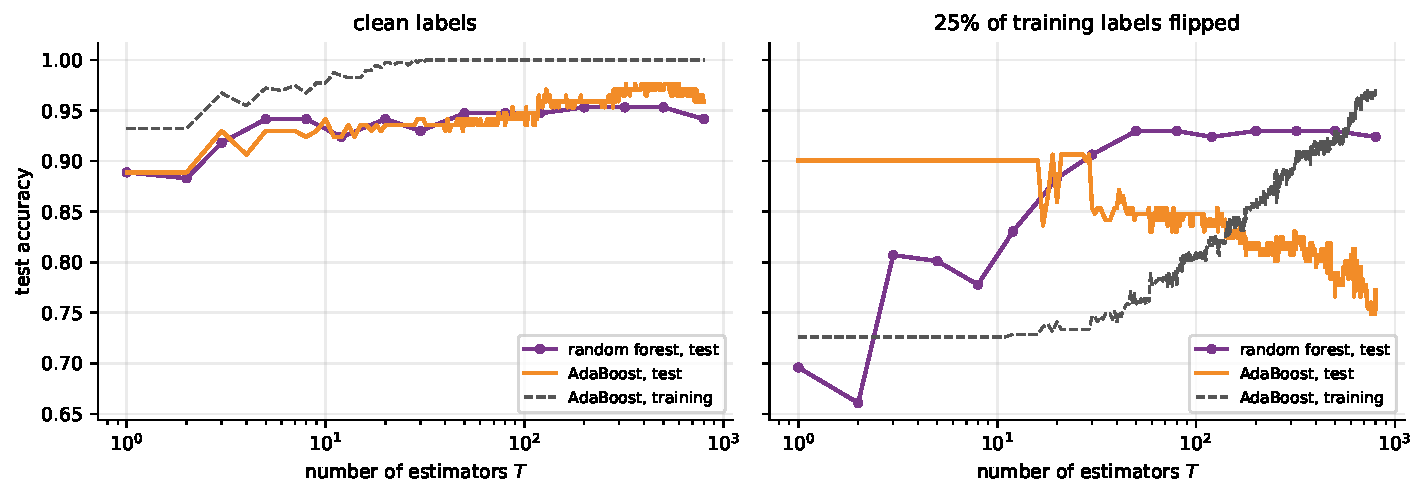
\includegraphics[width=0.98\textwidth]{nestimators.pdf}
  \caption{Test accuracy against the number of estimators, log scale. Left:
  clean labels. Right: $25\%$ of training labels flipped. The dashed grey line
  is AdaBoost's \emph{training} accuracy, which climbs in both panels.}
  \label{fig:nestimators}
\end{figure}

\subsection{All five, on three datasets}

\begin{lstlisting}
cvk = StratifiedKFold(5, shuffle=True, random_state=0)
models = [("single tree", DecisionTreeClassifier(random_state=0)),
          ("bagging 200", BaggingClassifier(DecisionTreeClassifier(random_state=0),
                                            n_estimators=200, random_state=0)),
          ("forest 200", RandomForestClassifier(n_estimators=200, random_state=0)),
          ("AdaBoost 200", AdaBoostClassifier(
              DecisionTreeClassifier(max_depth=1, random_state=0),
              n_estimators=200, random_state=0)),
          ("grad boosting", GradientBoostingClassifier(random_state=0))]
\end{lstlisting}
\begin{codeout}
                      wine     breast     digits
single tree         0.9273     0.9262     0.8592
bagging 200         0.9608     0.9579     0.9533
forest 200          0.9832     0.9667     0.9766
AdaBoost 200        0.9665     0.9754     0.8458
grad boosting       0.9494     0.9649     0.9655
\end{codeout}

Every ensemble beats the single tree on every dataset, with one exception, and
the exception is the interesting entry: AdaBoost scores $0.8458$ on
\texttt{digits}, \emph{below} the single tree's $0.8592$.

\begin{caution}[Boosted stumps are a two-class instrument]
\texttt{digits} has ten classes. SAMME requires each member to beat random
guessing on the weighted problem, that is $\varepsilon_t < 1 - 1/K = 0.9$, and
a depth-1 stump on a ten-class problem is barely above that line. The member
weights $\alpha_t$ come out tiny and the ensemble never gets going. Give
AdaBoost a depth-3 or depth-5 base learner on a multiclass problem, or use
gradient boosting, which scores $0.9655$ on the same data. The forest, which
needed no thought at all, scores $0.9766$.
\end{caution}

\begin{keyidea}
On tabular data, fit a random forest with default settings first. It needs no
feature scaling, no tuning and no separate validation split (use
\texttt{oob\_score=True}), it is top or near-top on all three datasets above,
and it tells you within seconds what accuracy is achievable. Then --- if the
labels are trustworthy and you have a tuning budget --- try gradient boosting to
beat it.
\end{keyidea}

\notesources{\AMLUnitVISources}

% =========================================================================
\section{Summary}
\label{sec:summary}

\begin{enumerate}[leftmargin=*]
  \item An \textbf{ensemble} combines many models. It helps only when the
    members are better than chance and \emph{fail on different rows}.
  \item \textbf{Condorcet's jury theorem.} Twenty-five independent voters at
    $p = 0.60$ vote correctly with probability $\mathbf{0.846232}$, a gain of
    $+0.2462$. Below $p = 0.5$ the same machinery makes things worse:
    $0.40$ becomes $0.0209$ with $101$ voters. At $p = 0.5$ nothing happens.
  \item \textbf{Correlation is the enemy.} With members held at exactly
    $60\%$ accuracy, a mean pairwise correlation of $0.126$ drops the vote
    from $0.8458$ to $\mathbf{0.6932}$; at correlation $1$ the committee is
    worth one member, $0.5993$.
  \item \textbf{The bootstrap.} A sample of $n$ drawn with replacement from
    $n$ contains $1 - (1 - 1/n)^n \to 1 - 1/e = \mathbf{0.632121}$ of the
    distinct rows. Measured at $n = 10\,000$: $0.632156$. At $n = 398$ the
    mean over $20\,000$ bags was $0.6325$ with standard deviation $0.0158$.
  \item \textbf{Out-of-bag.} The remaining $37\%$ gives free validation. Over
    twenty splits, OOB minus held-out was $\mathbf{+0.0008}$ with
    $p = 0.836$, and OOB had the \emph{smaller} standard deviation
    ($0.0054$ against $0.0137$).
  \item \textbf{Bagging reduces variance only.} Over $300$ resamples the
    variance of a deep tree fell $0.1230 \to \mathbf{0.0601}$ while bias$^2$
    moved $0.0005 \to 0.0002$. Bagging fifty \emph{stumps} halved the variance
    ($0.0281 \to 0.0147$) and left bias$^2$ at $0.1856 \to 0.1842$. So put
    deep learners in a bag, and do not bag an underfitting model.
  \item \textbf{The decorrelation identity.}
    $\operatorname{Var}(\bar T) = \rho\sigma^2 + \frac{1-\rho}{B}\sigma^2$.
    The first term contains no $B$, so once $B$ is large the only lever left
    is $\rho$.
  \item \textbf{Random forests} pull $\rho$ down with \texttt{max\_features}:
    $0.8261 \to 0.7945 \to 0.7010$ at $30, 5, 1$ features. Members get
    \emph{worse} ($0.9130 \to 0.8861$) and the ensemble peaks in the middle at
    $\mathbf{0.9532}$. Mean member $0.9120$, worst member $0.8480$, forest
    $0.9532$. OOB picked \texttt{max\_features=5} without seeing the test set.
  \item \textbf{Impurity importance is biased} towards high-cardinality
    columns. On a designed table two pure-noise $800$-level columns scored
    $0.3110$ and $0.3109$ against $0.2715$ for the only informative one.
    Permutation importance on held-out rows scored $\mathbf{+0.2136}$ against
    $+0.0081$ and $+0.0114$.
  \item \textbf{AdaBoost.} $\varepsilon_t = \sum_{h_t(x_i)\neq y_i} w_i$,
    $\alpha_t = \frac12\ln\frac{1-\varepsilon_t}{\varepsilon_t}$,
    $w_i \leftarrow w_i e^{-\alpha_t y_i h_t(x_i)}/Z_t$. On ten points:
    $\varepsilon = 0.3000, 0.2143, 0.1818$ and
    $\alpha = 0.4236, 0.6496, 0.7520$; three stumps that each get three points
    wrong combine to get $\mathbf{10}$ of $10$ right. scikit-learn reproduces
    every $\varepsilon$ and threshold; its weights are exactly $2\alpha$
    because SAMME omits the $\frac12$.
  \item \textbf{Gradient boosting} fits the residuals: $F_0 = 7.5$, then
    stumps on $y - F_{m-1}$, SSE $34 \to 2 \to 1.333 \to \mathbf{1.037}$,
    matching \texttt{GradientBoostingRegressor} to $0.00\mathrm{e}{+00}$. Use
    $\eta \approx 0.1$, not $1$.
  \item \textbf{Bagging versus boosting.} Parallel against sequential,
    variance against bias, robust against fragile. At $0\%$ label noise
    AdaBoost wins by $0.0088$; at $40\%$ the forest wins by $\mathbf{0.0602}$.
    With $25\%$ flipped labels AdaBoost peaks at $T = 19$ and then loses
    $0.1345$ while its training accuracy climbs to $0.9648$; the forest's
    peak-to-final drop is $0.0058$, one test row.
\end{enumerate}

% =========================================================================
\section{Practice questions}
\label{sec:practice}

Work these with a pen before running anything. Solutions with full working
follow in Section~\ref{sec:solutions}.

\begin{enumerate}[leftmargin=*]
  \item \textbf{Five independent voters.} Five classifiers, each correct with
    probability $p = 0.70$, independent. Compute the accuracy of their
    majority vote exactly. Then say what happens to your answer if the five
    are in fact perfectly correlated.

  \item \textbf{Bootstrap, by hand.} A training set has $n = 4$ rows. (a)
    Compute exactly the probability that a given row is \emph{absent} from a
    bootstrap sample, as a fraction and as a decimal. (b) Compute the expected
    number of distinct rows in the bag. (c) Compare with the large-$n$ limit
    and say whether $n = 4$ is above or below it, and why.

  \item \textbf{AdaBoost, round 1 by hand.} Five points, $x = 1,2,3,4,5$, with
    labels $y = +1, +1, -1, +1, -1$. The weak learner is a stump of the form
    ``predict $s$ if $x < \theta$, else $-s$'', with $\theta$ a half-integer.
    Starting from uniform weights $w_i = 0.2$: find the stump with the lowest
    weighted error, and compute $\varepsilon_1$, $\alpha_1$ and the five
    normalised weights after the update. Give $\alpha_1$ to four decimals.

  \item \textbf{AdaBoost, round 2 by hand.} Continue Question 3. Using the
    weights you computed, find the best stump for round 2 and compute
    $\varepsilon_2$ and $\alpha_2$. Then evaluate
    $F(x) = \alpha_1 h_1(x) + \alpha_2 h_2(x)$ at all five points and state how
    many the two-round ensemble classifies correctly.

  \item \textbf{The decorrelation identity.} A forest has $B = 200$ trees,
    each of variance $\sigma^2 = 1$, with mean pairwise correlation
    $\rho = 0.40$. (a) What is the variance of the forest's average? (b) How
    much would you gain by going to $B = 2000$? (c) How much would you gain by
    halving $\rho$ to $0.20$ at $B = 200$? Which is the better investment?

  \item \textbf{Reading an OOB score.} You fit a forest of $300$ trees and get
    \texttt{oob\_score\_} $= 0.9598$ and a held-out test score of $0.9298$ on
    $171$ rows. A classmate says the OOB score is dishonest and should be
    discarded. Using the numbers in Section~\ref{sec:oob}, give two reasons
    why that conclusion does not follow, and say what you would do to settle
    it.

  \item \textbf{Reading an importance table.} A colleague fits a forest to a
    customer dataset and sends you the top four features by
    \texttt{feature\_importances\_}: \texttt{transaction\_id} ($0.31$),
    \texttt{timestamp} ($0.24$), \texttt{amount} ($0.18$),
    \texttt{is\_weekend} ($0.02$). What do you tell them, what single
    computation do you ask for, and what do you expect it to show?

  \item \textbf{Which ensemble, and why.} You have $50\,000$ rows of tabular
    medical data labelled by three junior annotators whose pairwise agreement
    is about $85\%$. You have one afternoon and a sixteen-core machine.
    Forest or gradient boosting? Justify with at least two specific numbers
    from these notes.

  \item \textbf{Gradient boosting by hand.} Four points, $x = 1,2,3,4$ with
    $y = 2, 4, 8, 10$. Take $F_0 = \bar y$ and $\eta = 1$, and fit one
    depth-1 stump to the residuals (splitting between consecutive $x$ values,
    leaf value $=$ mean of the residuals in the leaf). Compute $F_1$ and the
    sum of squared errors before and after.

  \item \textbf{Why bagging fails here.} Explain, in terms of equation
    \eqref{eq:bv}, why bagging an ordinary least-squares linear regression on
    a large dataset buys almost nothing, and name one situation in which
    bagging a linear model \emph{would} help.
\end{enumerate}

% =========================================================================
\section{Solutions}
\label{sec:solutions}

\paragraph{1. Five independent voters.}
A majority of five is at least three. With $p = 0.7$, $q = 0.3$:
\[
  \binom{5}{3}p^3q^2 = 10(0.343)(0.09) = 0.30870,
\]
\[
  \binom{5}{4}p^4q = 5(0.2401)(0.3) = 0.36015,
  \qquad
  \binom{5}{5}p^5 = 0.16807.
\]
Sum: $0.30870 + 0.36015 + 0.16807 = \mathbf{0.83692}$. The vote gains
$+0.13692$ over a single member.

If the five are perfectly correlated they are the same classifier five times
over: whenever one is right all are right, so the majority is right exactly
when a member is, and the accuracy is $\mathbf{0.70}$. The entire gain
disappears, and no member's accuracy changed --- this is the copula table of
Section~\ref{sec:indep} in miniature.

\paragraph{2. Bootstrap by hand at $n = 4$.}
(a) Each of the four draws misses a fixed row with probability $3/4$, and the
draws are independent, so
\[
  \Pr[\text{absent}] = \Bigl(\frac{3}{4}\Bigr)^{4}
  = \frac{81}{256} = \mathbf{0.316406}.
\]
Therefore $\Pr[\text{present}] = 175/256 = 0.683594$.

(b) Let $I_j$ indicate that row $j$ is present. Expectation is linear whether
or not the $I_j$ are independent (they are not), so
\[
  \mathbb{E}[\#\text{distinct}] = \sum_{j=1}^{4}\Pr[I_j = 1]
  = 4 \times \frac{175}{256} = \frac{175}{64} = \mathbf{2.734375},
\]
a fraction of $0.683594$ of the four rows.

(c) The limit is $1 - 1/e = 0.632121$, so $n = 4$ is \emph{above} it. The
sequence $1 - (1-1/n)^n$ decreases towards the limit from above: at $n = 2$ it
is $0.75$, at $n = 4$ it is $0.6836$, at $n = 10$ it is $0.6513$. Small bags
retain a larger share of their rows because with few rows a given row gets a
relatively larger share of the draws.

\paragraph{3. AdaBoost round 1.}
Points $x = 1,\dots,5$, labels $y = +1, +1, -1, +1, -1$, weights all $0.2$.

Enumerate the stumps. With $s = +1$ (predict $+1$ below $\theta$):
\begin{center}
\begin{tabular}{lll}
  \toprule
  $\theta$ & predictions on $x = 1..5$ & wrong rows \\
  \midrule
  0.5 & $-,-,-,-,-$ & $1, 2, 4$ \quad (3) \\
  1.5 & $+,-,-,-,-$ & $2, 4$ \quad (2) \\
  2.5 & $+,+,-,-,-$ & $4$ \quad (1) \\
  3.5 & $+,+,+,-,-$ & $3, 4$ \quad (2) \\
  4.5 & $+,+,+,+,-$ & $3$ \quad (1) \\
  5.5 & $+,+,+,+,+$ & $3, 5$ \quad (2) \\
  \bottomrule
\end{tabular}
\end{center}
The $s = -1$ stumps are the complements and get $5 - k$ wrong, so their best
is $5 - 3 = 2$; they cannot beat one error. Two stumps tie at a single error:
$\theta = 2.5$ and $\theta = 4.5$. Take $\theta = 2.5$, $s = +1$ (the first
found by a left-to-right search). It is wrong only on $x = 4$, so
\[
  \varepsilon_1 = 0.2 = \mathbf{0.2000},
  \qquad
  \alpha_1 = \tfrac12\ln\frac{0.8}{0.2} = \tfrac12\ln 4
           = \tfrac12(1.386294) = \mathbf{0.693147}.
\]
(That $\alpha_1 = \ln 2$ exactly is a happy accident of $\varepsilon = 0.2$.)

Reweight. $e^{0.693147} = 2$ and $e^{-0.693147} = 0.5$, so the wrong row
becomes $0.2 \times 2 = 0.4$ and each of the four right rows becomes
$0.2 \times 0.5 = 0.1$. The normaliser is $Z_1 = 0.4 + 4(0.1) = 0.8$. Hence
\[
  w_4 = \frac{0.4}{0.8} = \mathbf{0.5},
  \qquad
  w_1 = w_2 = w_3 = w_5 = \frac{0.1}{0.8} = \mathbf{0.125}.
\]
Check: $0.5 + 4(0.125) = 1$. And note the misclassified row now carries total
weight exactly $0.5$, as the algorithm always arranges.

\paragraph{4. AdaBoost round 2.}
Weights are now $0.125, 0.125, 0.125, 0.5, 0.125$. Recount the weighted errors
of the same six thresholds, both polarities. The single point $x = 4$ carries
half the mass, so any stump that gets it wrong has $\varepsilon \geq 0.5$ and
is useless. Stumps that get $x = 4$ right:
\begin{itemize}
  \item $\theta = 3.5$, $s = -1$: predicts $-,-,-,+,+$; wrong on $1, 2, 5$;
    $\varepsilon = 0.125 \times 3 = 0.375$.
  \item $\theta = 4.5$, $s = +1$: predicts $+,+,+,+,-$; wrong on $3$;
    $\varepsilon = 0.125$.
  \item $\theta = 5.5$, $s = +1$: predicts $+,+,+,+,+$; wrong on $3, 5$;
    $\varepsilon = 0.25$.
  \item $\theta = 2.5$, $s = +1$ (round 1's stump): wrong on $4$;
    $\varepsilon = 0.5$ --- exactly chance, and $\alpha = 0$. The algorithm has
    made the previous member worthless, which is the point of the reweighting.
\end{itemize}
The best is $\theta = 4.5$, $s = +1$, with
\[
  \varepsilon_2 = \mathbf{0.1250},
  \qquad
  \alpha_2 = \tfrac12\ln\frac{0.875}{0.125} = \tfrac12\ln 7
           = \tfrac12(1.945910) = \mathbf{0.972955}.
\]

Now $F(x) = 0.693147\,h_1(x) + 0.972955\,h_2(x)$ with
$h_1 = (+,+,-,-,-)$ and $h_2 = (+,+,+,+,-)$:
\begin{center}
\begin{tabular}{ccccc}
  \toprule
  $x$ & $h_1$ & $h_2$ & $F(x)$ & $y$ \\
  \midrule
  1 & $+1$ & $+1$ & $+1.666102$ & $+1$ \\
  2 & $+1$ & $+1$ & $+1.666102$ & $+1$ \\
  3 & $-1$ & $+1$ & $+0.279808$ & $-1$ \\
  4 & $-1$ & $+1$ & $+0.279808$ & $+1$ \\
  5 & $-1$ & $-1$ & $-1.666102$ & $-1$ \\
  \bottomrule
\end{tabular}
\end{center}
Signs are $+,+,+,+,-$, so the ensemble gets $x = 1, 2, 4, 5$ right and $x = 3$
wrong: \textbf{four of five}. Both individual stumps also got four of five, so
two rounds have not yet improved on a single stump here --- which is honest and
worth noticing. The reason is visible in the table: $h_1$ and $h_2$ disagree
only on $x = 3$ and $x = 4$, and $\alpha_2 > \alpha_1$ so $h_2$ wins both.
Points $3$ and $4$ are adjacent in $x$ with opposite labels, and no combination
of two thresholds can separate them from their neighbours; a third round is
needed.

\paragraph{5. The decorrelation identity.}
(a) $\rho + (1-\rho)/B = 0.40 + 0.60/200 = 0.40 + 0.0030 = \mathbf{0.4030}$.

(b) At $B = 2000$: $0.40 + 0.60/2000 = 0.40030$. The gain is $0.00270$ --- ten
times the trees for a variance reduction of about a quarter of one percent.

(c) At $\rho = 0.20$, $B = 200$: $0.20 + 0.80/200 = \mathbf{0.2040}$. The gain
is $0.1990$, roughly \textbf{seventy-four times} the gain from the ten-fold
increase in $B$.

Decorrelating is overwhelmingly the better investment, and that single
comparison is the entire justification for \texttt{max\_features}. Once $B$ is
in the hundreds, the $(1-\rho)/B$ term is already negligible and all that is
left is $\rho\sigma^2$.

\paragraph{6. Reading an OOB score.}
Two reasons the conclusion does not follow.

First, \textbf{one split is one observation}. The held-out score here is
computed on $171$ rows, so its standard deviation across splits is $0.0137$
(Section~\ref{sec:oob}); a gap of $0.0300$ is about two standard deviations of
a single noisy measurement, which happens regularly. Repeated over twenty
splits the mean gap was $+0.0008$ with $p = 0.836$.

Second, the direction of any systematic OOB bias is \emph{pessimistic}, not
optimistic: each OOB prediction uses only the $\approx 37\%$ of members that
did not see the row, so OOB measures a smaller ensemble than the one you
deploy. There is no mechanism that would make OOB systematically flatter you.

To settle it: repeat the split with twenty or thirty different
\texttt{random\_state} values, collect both scores each time, and do a paired
$t$-test on the differences, as in Section~\ref{sec:oob}.

\paragraph{7. Reading an importance table.}
\texttt{transaction\_id} is an identifier: it takes a distinct value on every
row, carries no information about anything, and is the exact case
Section~\ref{sec:imp} was written about. \texttt{timestamp} is close behind ---
thousands of distinct values, and very likely a leak besides. That these two
top the list is not evidence that they matter; it is evidence that the metric
is MDI. Note also that \texttt{is\_weekend}, a two-level column, is at the
bottom \emph{by construction}: two levels means two candidate splits.

Ask for one computation: \texttt{permutation\_importance} on a
\textbf{held-out} split, with \texttt{n\_repeats=30}, reporting the mean and
the standard deviation. Expect \texttt{transaction\_id} to come out at
approximately $0.0000$ with a tiny standard deviation, as
\texttt{noise\_uid(569)} did in Demonstration~1. Then have them drop the
identifier and refit; if the accuracy is unchanged, the case is closed.

\paragraph{8. Which ensemble, and why.}
A \textbf{random forest}, and it is not close.

Pairwise annotator agreement of $85\%$ means the label column carries
double-digit noise. Section~\ref{sec:vs} measures exactly this: at $10\%$
flipped labels the forest led AdaBoost by $0.0374$ and at $20\%$ by $0.0579$,
and with $25\%$ flipped labels boosting peaked at $T = 19$ and then gave back
$0.1345$ while its training accuracy climbed to $0.9648$ on labels that were a
quarter wrong. Boosting's reweighting rule cannot distinguish ``hard row''
from ``wrong label''.

The other two constraints point the same way. One afternoon is not a tuning
budget, and gradient boosting has at least three interacting hyperparameters
($\eta$, depth, $T$) while a forest has essentially none --- the defaults were
at or near the top of every column of the three-dataset table. And sixteen
cores are worth sixteen times as much to a forest, whose trees are
independent, as to boosting, which is inherently sequential. Use
\texttt{oob\_score=True} so the whole $50\,000$ rows train the model.

\paragraph{9. Gradient boosting by hand.}
$F_0 = \bar y = (2 + 4 + 8 + 10)/4 = 6$. Residuals: $-4, -2, +2, +4$. Initial
$\mathrm{SSE} = 16 + 4 + 4 + 16 = \mathbf{40}$.

Try the three splits, computing the SSE of the residuals about their leaf
means:
\begin{center}
\begin{tabular}{llll}
  \toprule
  split & left leaf (mean) & right leaf (mean) & SSE of residuals \\
  \midrule
  $x < 1.5$ & $\{-4\}$ ($-4$) & $\{-2, 2, 4\}$ ($1.3333$)
    & $0 + 24.6667 = 24.6667$ \\
  $x < 2.5$ & $\{-4, -2\}$ ($-3$) & $\{2, 4\}$ ($3$)
    & $2 + 2 = \mathbf{4}$ \\
  $x < 3.5$ & $\{-4, -2, 2\}$ ($-1.3333$) & $\{4\}$ ($4$)
    & $24.6667 + 0 = 24.6667$ \\
  \bottomrule
\end{tabular}
\end{center}
The stump splits at $x < 2.5$ with leaf values $-3$ and $+3$. So
\[
  F_1 = 6 + (-3, -3, +3, +3) = (3, 3, 9, 9),
\]
and the new residuals are $2 - 3 = -1$, $4 - 3 = +1$, $8 - 9 = -1$,
$10 - 9 = +1$, giving
\[
  \mathrm{SSE} = 1 + 1 + 1 + 1 = \mathbf{4}.
\]
One stump took the error from $40$ to $4$, a reduction of $90\%$ --- and note
that the residual SSE after the split is exactly the ``SSE of residuals''
column, which is what the tree was minimising.

\paragraph{10. Why bagging fails on OLS.}
Bagging only moves the variance term of equation \eqref{eq:bv}, and on a large
dataset an OLS fit has almost no variance to move. The coefficient estimator
$\hat\beta = (X^\top X)^{-1}X^\top y$ has covariance
$\sigma^2 (X^\top X)^{-1}$, which shrinks like $1/n$; with $n$ large, a
bootstrap resample produces very nearly the same $\hat\beta$, so the members of
the bag are almost identical --- $\rho$ near $1$ in equation
\eqref{eq:corravg}, and Section~\ref{sec:indep}'s last row applies. Meanwhile
the bias of a linear model on a non-linear truth is untouched, because bagging
cannot touch bias.

This is Breiman's own condition restated: bagging helps \emph{unstable}
predictors, and OLS with $n \gg p$ is about as stable as a method gets.

Bagging a linear model \emph{would} help when the fit is unstable: $p$
comparable to or larger than $n$, severe multicollinearity, or a fitting
procedure with a discrete choice in it. Breiman's 1996 paper makes exactly
this point with \emph{subset selection} in linear regression --- the choice of
which variables enter is a discontinuous function of the data, so it jumps
around under resampling, and bagging it does help.

% =========================================================================
\section{References and further reading}
\label{sec:refs}

All links were checked on 23 August 2026. Free resources are marked
\textbf{[free]}.

\subsection*{Textbooks}

\begin{itemize}[leftmargin=*]
  \item Han, Kamber and Pei, \emph{Data Mining: Concepts and Techniques}, 3rd
    edition, Morgan Kaufmann, 2012. \textbf{The prescribed text for this
    lecture.} \S8.6 techniques to improve classification accuracy ---
    \S8.6.1 introduces ensemble methods and the vocabulary the examination
    uses; \S8.6.2 is bagging, with the algorithm in the same form as
    Section~\ref{sec:bag}; \S8.6.3 is boosting and AdaBoost, including the
    weight update of equation \eqref{eq:reweight}; \S8.6.4 is random forests;
    \S8.6.5 is class-imbalanced data. \S8.5.4 on model selection and the
    paired $t$-test is the background for Section~\ref{sec:oob}.
  \item James, Witten, Hastie, Tibshirani and Taylor, \emph{An Introduction to
    Statistical Learning with Python}. \textbf{[free]} \S8.2 is this lecture
    almost exactly --- \S8.2.1 bagging, with the $2/3$ figure and out-of-bag
    error estimation; \S8.2.2 random forests and the decorrelation argument of
    Section~\ref{sec:rf}; \S8.2.3 boosting and its three tuning parameters;
    \S8.2.5 variable importance. \S5.2 is the bootstrap itself.
    \url{https://www.statlearning.com/}
  \item M\"uller and Guido, \emph{Introduction to Machine Learning with
    Python}, O'Reilly, 2016. \S2.3.6 ensembles of decision trees --- random
    forests (building them, analysing them, the strengths and weaknesses
    section) and gradient boosted regression trees, with the
    \texttt{learning\_rate} discussion of Section~\ref{sec:boost}. Notebooks
    \textbf{[free]}:
    \url{https://github.com/amueller/introduction_to_ml_with_python}
  \item Hastie, Tibshirani and Friedman, \emph{The Elements of Statistical
    Learning}, 2e, Springer. \textbf{[free]} \S8.7 bagging; Chapter 10 on
    boosting, with \S10.1 giving the AdaBoost.M1 algorithm exactly as
    Section~\ref{sec:boost} states it and \S10.4 showing that it is forward
    stagewise fitting of an exponential loss; Chapter 15 on random forests,
    with \S15.2 the definition, \S15.4.1 the variance-and-decorrelation
    argument behind equation \eqref{eq:corravg}, and \S15.3.2 variable
    importance. \url{https://hastie.su.domains/ElemStatLearn/}
  \item Zhi-Hua Zhou, \emph{Ensemble Methods: Foundations and Algorithms},
    Chapman and Hall/CRC, 2012. The monograph on the subject. Chapter 2
    boosting, Chapter 3 bagging, Chapter 4 combination methods, Chapter 5
    diversity --- Chapter 5 is the formal treatment of the correlation
    argument this lecture makes empirically in Section~\ref{sec:indep}.
\end{itemize}

\subsection*{Online courses}

\begin{sloppypar}
\begin{itemize}[leftmargin=*]
  \item \textbf{NPTEL, Introduction to Machine Learning} --- Prof.\ Balaraman
    Ravindran, IIT Madras; the reference course for the semester. The
    ensembles week covers bagging, boosting, AdaBoost and random forests in
    the notation used here. \textbf{[free]}
    \url{https://nptel.ac.in/courses/106106139}
  \item \textbf{NPTEL, Data Mining} --- Prof.\ Pabitra Mitra, IIT Kharagpur.
    Follows the Han--Kamber--Pei chapter structure, so its classification
    weeks map onto \S8.6 directly. \textbf{[free]}
    \url{https://nptel.ac.in/courses/106105174}
  \item \textbf{NPTEL, Introduction to Machine Learning} --- Prof.\ Sudeshna
    Sarkar, IIT Kharagpur. A second treatment of ensembles worked at the
    board, if the first does not land. \textbf{[free]}
    \url{https://nptel.ac.in/courses/106105152}
  \item \textbf{SWAYAM} --- the national portal hosting NPTEL, with
    certification cycles. \textbf{[free]} \url{https://swayam.gov.in/}
  \item \textbf{Kaggle Learn, Intro to Machine Learning} --- lesson 6 is
    random forests in the browser, five minutes after the decision-tree
    lessons. \textbf{[free]}
    \url{https://www.kaggle.com/learn/intro-to-machine-learning}
  \item \textbf{Google Machine Learning Crash Course} --- the ``Overfitting''
    and ``Generalization'' modules are the background for
    Section~\ref{sec:vs}. \textbf{[free]}
    \url{https://developers.google.com/machine-learning/crash-course}
\end{itemize}
\end{sloppypar}

\subsection*{Videos}

\begin{itemize}[leftmargin=*]
  \item StatQuest with Josh Starmer, \emph{StatQuest: Random Forests Part 1 -
    Building, Using and Evaluating} --- bagging, the random feature subset and
    the out-of-bag estimate at a whiteboard. Watch this one first.
    \textbf{[free]} \url{https://youtu.be/J4Wdy0Wc_xQ}
  \item StatQuest with Josh Starmer, \emph{Bootstrapping Main Ideas!!!} --- the
    bootstrap on its own, before any ensemble, which is the right order if
    Section~\ref{sec:632} did not land. \textbf{[free]}
    \url{https://youtu.be/Xz0x-8-cgaQ}
  \item StatQuest with Josh Starmer, \emph{AdaBoost, Clearly Explained} --- the
    stumps, the amount of say (his name for $\alpha_t$) and the reweighting,
    drawn out step by step. It is the video companion to
    Section~\ref{sec:adahand}. \textbf{[free]}
    \url{https://youtu.be/LsK-xG1cLYA}
  \item StatQuest with Josh Starmer, \emph{Gradient Boost Part 1 (of 4):
    Regression Main Ideas} --- fitting the residuals, with the learning rate.
    Parts 2 to 4 do the mathematics and the classification case.
    \textbf{[free]} \url{https://youtu.be/3CC4N4z3GJc}
\end{itemize}

\subsection*{Documentation and interactive explainers}

\begin{itemize}[leftmargin=*]
  \item MLU-Explain, \emph{The Random Forest Algorithm} --- Amazon's scrollable
    explainer, and it opens with Condorcet's jury theorem exactly as
    Section~\ref{sec:jury} does, with sliders for the number of trees and each
    tree's accuracy. The ``Variance in Predictions'' grid is
    Section~\ref{sec:indep} made visual. \textbf{[free]}
    \url{https://mlu-explain.github.io/random-forest/}
  \item MLU-Explain, \emph{The Bias Variance Tradeoff} --- the decomposition of
    equation \eqref{eq:bv} with interactive model realisations, which is what
    Figure~\ref{fig:biasvar} shows statically. \textbf{[free]}
    \url{https://mlu-explain.github.io/bias-variance/}
  \item scikit-learn user guide, \emph{1.11. Ensembles: Gradient boosting,
    random forests, bagging, voting, stacking} --- the reference for every
    class used in these notes, including the SAMME weight that explains the
    factor of two in Section~\ref{sec:boost}. \textbf{[free]}
    \url{https://scikit-learn.org/stable/modules/ensemble.html}
  \item scikit-learn user guide, \emph{5.2. Permutation feature importance} ---
    \S5.2.1 is the algorithm of Section~\ref{sec:imp}, \S5.2.2 states the
    high-cardinality bias of impurity importance in the documentation's own
    words, and \S5.2.3 is the correlated-features caveat. \textbf{[free]}
    \url{https://scikit-learn.org/stable/modules/permutation_importance.html}
  \item scikit-learn example, \emph{Permutation Importance vs Random Forest
    Feature Importance (MDI)} --- the same demonstration as
    Section~\ref{sec:imp}, on the Titanic data with a planted random
    categorical column. \textbf{[free]}
    \url{https://scikit-learn.org/stable/auto_examples/inspection/plot_permutation_importance.html}
\end{itemize}

\subsection*{Articles}

\begin{itemize}[leftmargin=*]
  \item L.\ Breiman, ``Bagging predictors'', \emph{Machine Learning}
    \textbf{24}(2), 123--140, 1996. The paper that named bagging. Its abstract
    contains the sentence Section~\ref{sec:bag} quotes --- \emph{the vital
    element is the instability of the prediction method} --- and \S4 is the
    subset-selection experiment behind the answer to Practice Question 10.
    \url{https://doi.org/10.1007/BF00058655}
  \item L.\ Breiman, ``Random Forests'', \emph{Machine Learning} \textbf{45}(1),
    5--32, 2001. The abstract states the result of Section~\ref{sec:rf}
    directly: the generalisation error ``depends on the strength of the
    individual trees in the forest and the correlation between them'', and a
    random feature selection gives error rates comparable to AdaBoost ``but
    more robust with respect to noise'' --- which is what
    Section~\ref{sec:vs} measures. \url{https://doi.org/10.1023/A:1010933404324}
  \item Y.\ Freund and R.\ E.\ Schapire, ``A decision-theoretic generalization
    of on-line learning and an application to boosting'', \emph{Journal of
    Computer and System Sciences} \textbf{55}(1), 119--139, 1997. The AdaBoost
    paper. \S3 is the algorithm of Section~\ref{sec:boost} and the derivation
    of $\alpha_t$ as the minimiser of the normaliser $Z_t$.
    \url{https://doi.org/10.1006/jcss.1997.1504}
  \item J.\ H.\ Friedman, ``Greedy function approximation: a gradient boosting
    machine'', \emph{Annals of Statistics} \textbf{29}(5), 1189--1232, 2001.
    The paper that made ``fit the residuals'' into ``descend the gradient in
    function space''; \S3 is the squared-error case worked in
    Section~\ref{sec:boost} and \S5 introduces the shrinkage parameter $\eta$.
    \url{https://doi.org/10.1214/aos/1013203451}
  \item C.\ Strobl, A.-L.\ Boulesteix, A.\ Zeileis and T.\ Hothorn, ``Bias in
    random forest variable importance measures: illustrations, sources and a
    solution'', \emph{BMC Bioinformatics} \textbf{8}:25, 2007. \textbf{[free]}
    The formal version of Section~\ref{sec:imp}: why impurity importance
    prefers high-cardinality predictors, and what to do instead.
    \url{https://doi.org/10.1186/1471-2105-8-25}
\end{itemize}

\notesources{\AMLUnitVISources}

\end{document}
